\chapter{塑造神经系统} \label{chap:chap45}

在脊椎动物神经系统的发育过程中会产生大量的神经元和神经胶质细胞。
不同类型的神经元在离散的解剖位置发育,获得不同的形态学形式,并与特定的靶细胞群建立联系。
它们的多样性远远超过身体任何其他器官中的细胞。
例如,视网膜有几十种中间神经元,脊髓有一百多种运动神经元。
目前,哺乳动物中枢神经系统中神经元类型的真实数量仍然未知,但肯定超过一千种。
神经胶质类型的数量就更不清楚了。
在直到最近还被认为是相当均匀的星形胶质细胞和少突胶质细胞类别中发现了意想不到的异质性。


神经元类型的多样性是哺乳动物神经系统令人印象深刻的计算特性的基础。
然而,正如我们在本章和后续章节中所描述的那样,驱动神经系统分化的发育原则是从用于指导其他组织发育的原则中借鉴和借鉴的。
从某种意义上说,神经系统的发育仅代表了贯穿所有发育生物学的基本挑战的详尽示例:如何将单个细胞(受精卵)转化为成熟生物体所特有的高度分化的细胞类型。
只有在后期阶段,当神经元形成复杂的回路并且经验改变它们的连接时,神经发育的原则才会与其他器官的原则不同。


早期发育原则不仅在组织之间而且在物种和门之间也是保守的。
事实上,我们对脊椎动物神经发育的细胞和分子基础的了解大部分来自所谓的简单生物的遗传研究,最著名的是果蝇 Drosophila melanogaster 和蠕虫 Caenorhabditis elegans。
然而,由于研究神经发育的主要目标是解释神经系统的组装如何成为人类行为和大脑障碍的基础,因此我们对神经系统发育规则和原则的描述主要集中在脊椎动物身上。



\section{神经管起源于外胚层}

脊椎动物胚胎来自受精卵。
细胞分裂最初形成一个细胞球,称为桑葚胚,然后空心形成囊胚。
接下来,折叠和生长产生原肠胚,这是一种具有极性的结构(背腹侧和前后)和三层细胞——内胚层、中胚层和外胚层(图 \ref{fig:45_1}A)。


\begin{figure}[htbp]
	\centering
	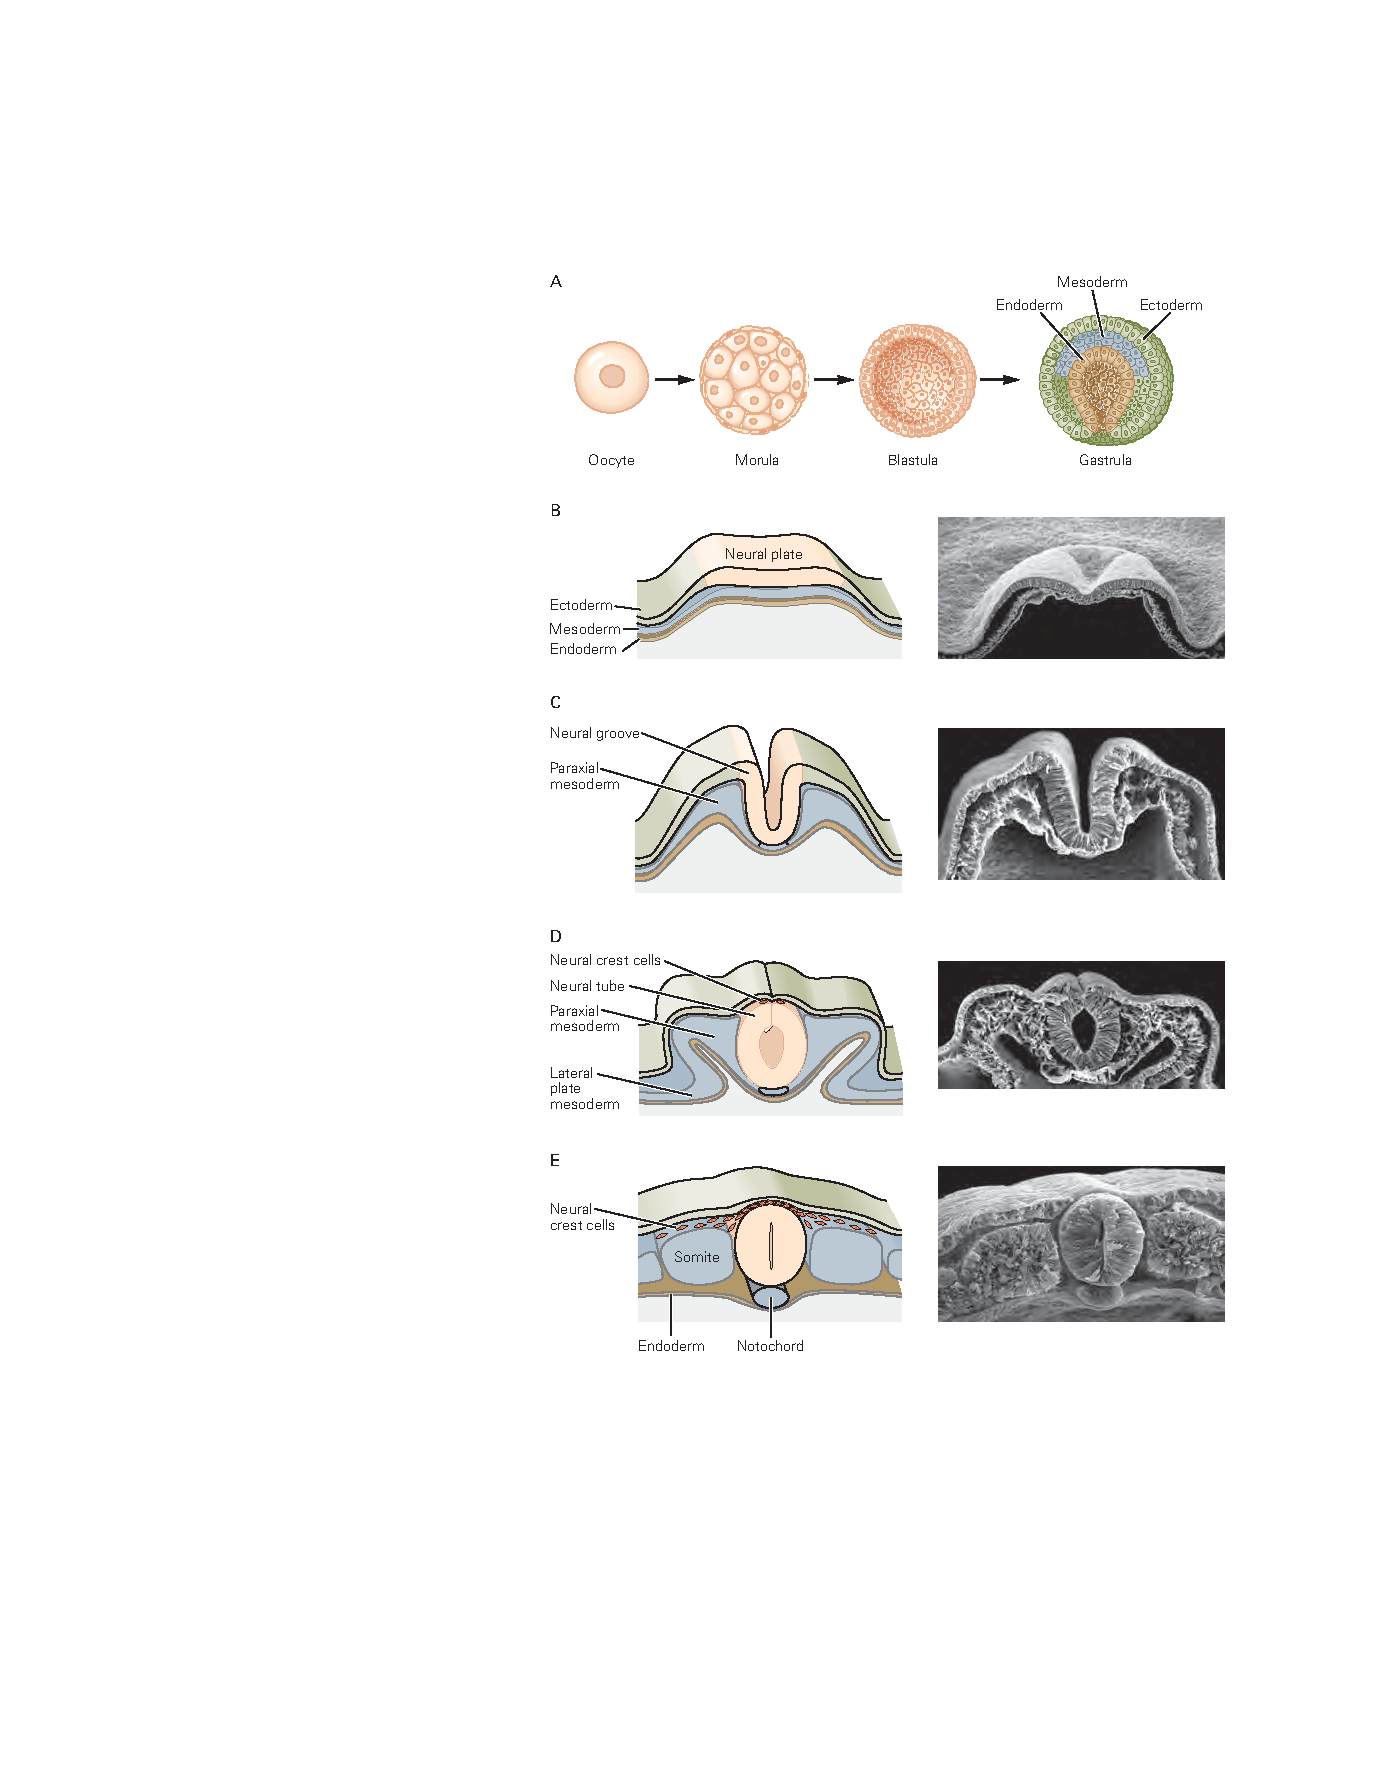
\includegraphics[width=0.65\linewidth]{chap45/fig_45_1}
	\caption{神经板折叠形成神经管。 (经 G. Schoenwolf 许可转载的小鸡神经管扫描电子显微照片。) A. 卵子受精后,细胞分裂依次产生桑葚胚、囊胚和原肠胚。 三个生殖细胞层——外胚层、中胚层和内胚层——在原肠胚形成过程中形成。 B. 一条外胚层变成神经板,是中枢和周围神经系统的前身。 C. 神经板在中线处弯曲形成神经沟。 D. 背侧神经皱襞闭合形成神经管。 E. 神经管位于脊索上方,两侧是体节,体节是产生肌肉和软骨的卵圆形中胚层细胞群。 神经管和覆盖的外胚层之间交界处的细胞被放在一边成为神经嵴。}
	\label{fig:45_1}
\end{figure}


内胚层是最里面的胚层,后来产生肠道、肺、胰腺和肝脏。
中胚层是产生肌肉、结缔组织和大部分血管系统的中间胚层。
外胚层是最外层。
大部分外胚层产生皮肤,但一条狭窄的中央条带变平成为神经板(图 \ref{fig:45_1}B)。
中枢和周围神经系统是从神经板产生的。


神经板形成后不久,它开始内陷,形成神经沟。
然后褶皱加深并最终与外胚层的其余部分分离,形成神经管,通过称为神经形成的过程(图 \ref{fig:45_1}C,D)。
神经管的尾部区域产生脊髓,而喙部区域成为大脑。
当神经管关闭时,其与上覆外胚层交界处的细胞被搁置一旁,成为神经嵴,最终产生自主神经系统和感觉神经系统,以及几种非神经细胞类型(图 \ref{fig:45_1}E)。



\section{分泌信号促进神经细胞命运}

神经板形成后不久,它开始内陷,形成神经沟。
然后褶皱加深并最终与外胚层的其余部分分离,形成神经管,通过称为神经形成的过程(图 \ref{fig:45_1}C,D)。
神经管的尾部区域产生脊髓,而喙部区域成为大脑。
当神经管关闭时,其与上覆外胚层交界处的细胞被搁置一旁,成为神经嵴,最终产生自主神经系统和感觉神经系统,以及几种非神经细胞类型(图 \ref{fig:45_1}E)。


这项工作的大部分重点是寻找控制外胚层细胞命运的信号。
我们现在知道,两大类蛋白质共同作用促进外胚层细胞分化为神经细胞。
第一种是诱导因子,即附近细胞分泌的信号分子。
其中一些因子可自由扩散并在远处发挥作用,但其他因子则被束缚在细胞表面并在局部发挥作用。
第二种是使细胞能够对诱导因子作出反应的表面受体。
这些受体的激活会触发编码细胞内蛋白质(转录因子、酶和细胞骨架蛋白)的基因的表达,从而推动外胚层细胞沿着成为神经细胞的途径前进。


细胞对感应信号作出反应的能力,称为它的能力,取决于它表达的受体、转导分子和转录因子的确切库。
因此,细胞的命运不仅取决于它所暴露的信号——它在胚胎中发现自己的时间和地点的结果——而且还取决于它表达的基因概况,这是其先前发育历史的结果。
我们将在后续章节中看到,局部感应信号和内在细胞反应性的相互作用在神经发育的几乎每一步中都是显而易见的。



\subsection{神经板的发育是由来自组织者区域的信号诱导的}

特定信号负责触发神经板形成的发现是理解神经系统模式机制的第一个重大进展。
1924 年,汉斯·斯佩曼 (Hans Spemann) 和希尔德·曼戈尔德 (Hilde Mangold) 做出了非凡的观察,即神经板与未定型外胚层的分化取决于一组被称为组织者区域的特殊细胞分泌的信号。


他们的实验涉及将小块组织从一个两栖动物胚胎移植到另一个胚胎。
最有说服力的是胚孔背唇的移植,它注定要形成背中胚层,从正常的背侧位置移植到宿主胚胎的腹侧。
背唇位于背外胚层下方,该区域通常会产生背表皮,包括神经板(图 \ref{fig:45_2})。
他们将有色胚胎的组织移植到无色素的宿主中,使他们能够区分供体细胞和宿主细胞的位置和命运。


\begin{figure}[htbp]
	\centering
	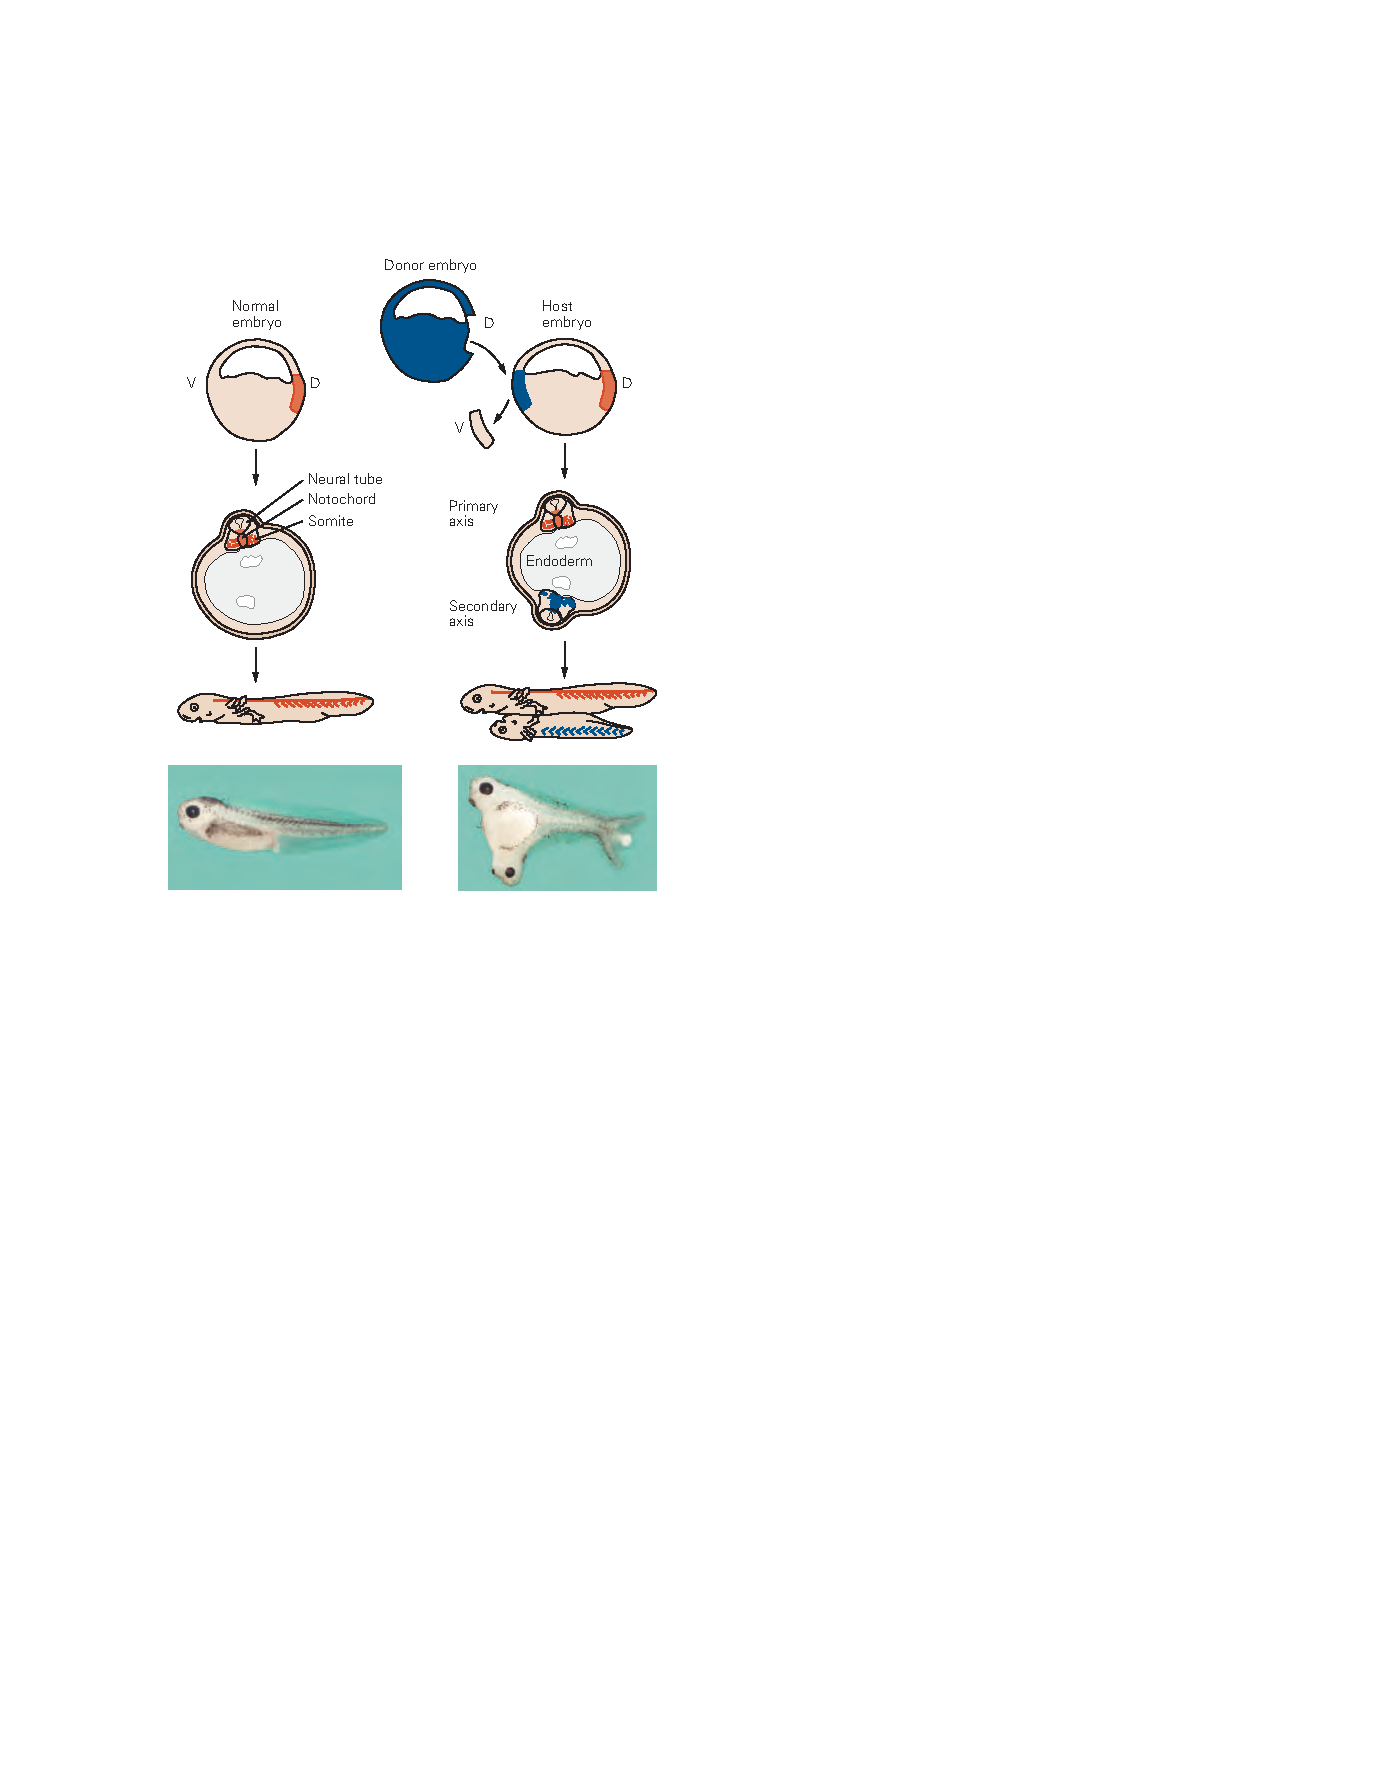
\includegraphics[width=0.5\linewidth]{chap45/fig_45_2}
	\caption{来自组织者区域的信号诱导第二个神经管。 (显微照片经许可转载自 Eduardo de Robertis。)左图:在正常青蛙中,来自组织区(背胚孔唇)的胚胎细胞分布在脊索、底板和体节上。 右图:Spemann 和 Mangold 将早期原肠胚期胚胎的背侧胚孔唇移植到宿主胚胎的一个区域,该区域通常会产生腹侧表皮。 来自移植细胞的信号诱导第二个胚胎轴,其中包括一个几乎完整的神经管。 供体组织来自有色素的胚胎,而宿主组织没有色素,因此可以通过颜色监测移植细胞的命运。 移植细胞本身仅对宿主胚胎的脊索、底板和体节有贡献。 随着胚胎的成熟,次级神经管发育成一个完整的神经系统。 在显微照片中显示的非洲爪蟾胚胎中,第二个神经轴是通过注射骨形态发生蛋白 (BMP) 拮抗剂诱导的,实际上替代了组织者信号(图 \ref{fig:45_3})。 初级神经轴也很明显。 (缩写:D,背侧;V,腹侧。)}
	\label{fig:45_2}
\end{figure}


\begin{figure}[htbp]
	\centering
	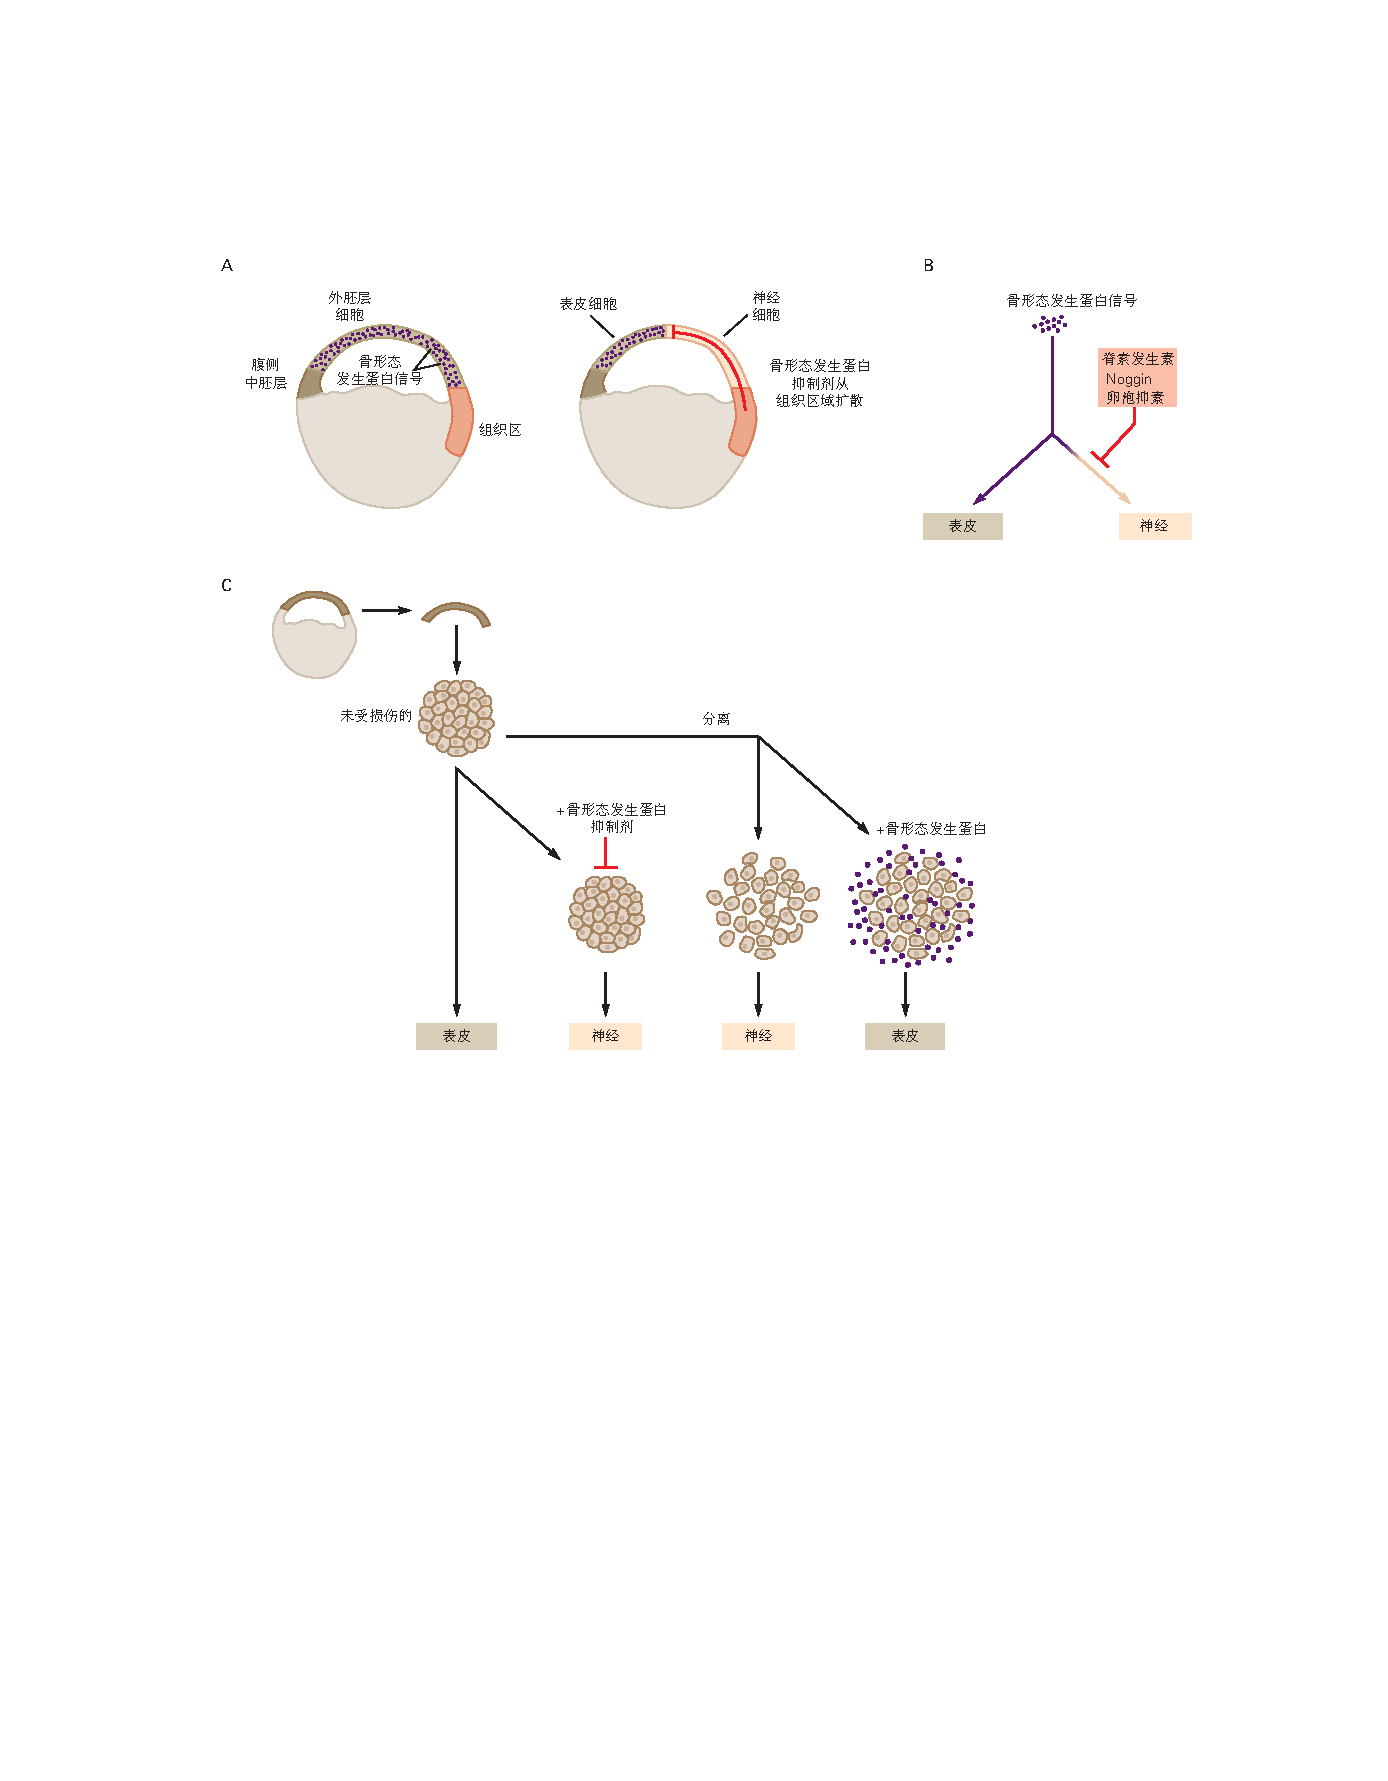
\includegraphics[width=0.9\linewidth]{chap45/fig_45_3}
	\caption{骨形态发生蛋白 (BMP) 信号的抑制启动神经感应。 A. 在爪蟾蛙胚胎中,来自组织者区域(红线)的信号通过外胚层传播以诱导神经组织。 超出组织者信号范围的外胚层组织产生表皮。 B. 从组织者区域分泌的 BMP 抑制剂(包括头蛋白、卵泡抑素和脊索蛋白)与 BMP 结合并阻断外胚层细胞获得表皮命运的能力,从而促进神经特性。 C. 外胚层细胞根据是否存在 BMP 信号获得神经或表皮特征。 当外胚层细胞聚集体暴露于 BMP 信号时,它们会分化为表皮组织。 当 BMP 信号被阻断时,无论是通过将外胚层组织分离成单个细胞,还是通过将 BMP 抑制剂添加到外胚层细胞聚集体中,细胞都会分化为神经组织。}
	\label{fig:45_3}
\end{figure}


Spemann 和 Mangold 发现,从胚孔背唇移植的细胞遵循它们的正常发育程序,产生中线中胚层组织,如体节和脊索。
但是移植的细胞也引起了邻近宿主胚胎腹侧外胚层细胞命运的显着变化。
宿主外胚层细胞被诱导形成几乎完整的神经系统副本(图 \ref{fig:45_2})。
因此,他们称供体组织为组织者。
Spemann 和 Mangold 继续证明胚孔的背唇是唯一具有这种“组织”作用的组织。


这些开创性研究还表明,“归纳”在神经发育中起着至关重要的作用。
诱导是一种过程,通过该过程,一个组织的细胞在两个接近的区域指导相邻细胞的发育。
重要的是它提供了一种机制,来自一个组织的信号可以通过该机制导致第二个组织的细分。
在这种情况下,中胚层诱导外胚层的一部分变成神经板,最终变成神经系统,而其余部分继续变成上皮,最后变成皮肤。
由此形成的新并置原则上可以为后续的归纳和细分级联奠定基础。
事实上,我们将看到现在已知神经管模式的许多方面取决于局部组织中心通过原则上类似于经典组织者区域的行为分泌的信号。



\subsection{神经诱导是由肽生长因子及其抑制剂介导的}

在 Spemann 和 Mangold 的开创性研究之后的几十年里,神经诱导剂的鉴定构成了发育生物学的圣杯。
直到 1980 年代,这项研究才取得了一些成功,当时分子生物学的出现和早期神经组织更好的标记物的可用性导致我们对神经诱导及其化学介质的理解取得了突破。


第一个进展来自一个简单的发现:当早期外胚层分离成单个分离细胞时,有效地阻止了细胞间信号传导,细胞在没有添加因子的情况下很容易获得神经特性(图 \ref{fig:45_3}A)。
这一发现令人惊讶的含义是,外胚层细胞的“默认”命运是神经分化,而这种命运是通过外胚层细胞之间的信号传递来阻止的。
在这个模型中,长期以来备受追捧的“诱导剂”实际上是一种“去阻遏物”:它阻止外胚层抑制神经命运。


这些想法立即引发了两个进一步的问题。
什么外胚层信号抑制神经分化,组织者组织提供什么来克服阻遏物的影响?
青蛙和小鸡的神经诱导研究现已为这些问题提供了答案。


在没有来自组织者的信号的情况下,外胚层细胞合成并分泌骨形态发生蛋白 (BMP),这是转化生长因子 β (TGFβ) 相关蛋白大家族的成员。
BMP 通过外胚层细胞上的丝氨酸/苏氨酸激酶类受体起作用,抑制神经分化的潜力并促进表皮分化(图 43-3B)。
BMP 作为神经抑制因子的作用的关键证据来自实验,在实验中,BMP 受体的截短版本被发现会触发非洲爪蟾胚胎中的神经组织分化。
相反,外胚层细胞暴露于 BMP 信号转导促进分化为表皮细胞(图 \ref{fig:45_3}C)。


BMP 作为神经元分化抑制因子的鉴定反过来表明,组织者可能通过分泌拮抗 BMP 信号传导的因子来诱导外胚层细胞的神经分化。
对这一想法的直接支持来自组织者区域的细胞表达许多充当 BMP 拮抗剂的分泌蛋白的发现。
这些蛋白质包括 noggin、chordin、follistatin,甚至一些变异的 BMP 蛋白质。
这些蛋白质中的每一种都具有诱导外胚层细胞分化为神经组织的能力(图 \ref{fig:45_3}B)。
因此,没有单一的神经诱导剂。
事实上,诱导需要多种蛋白质,正如后来发现的那样,外胚层细胞暴露于成纤维细胞生长因子 (FGF) 也是神经分化的必要步骤。


总之,这些研究为神经诱导的细胞现象提供了分子解释。 尽管该途径的许多细节仍有待阐明,并且物种之间的一些机制差异仍然令人费解,但在 Spemann 和 Mangold 发现组织者近一个世纪后,神经发育的一个关键章节现在已经得出了令人满意的结论。



\section{神经管的 Rostrocaudal 模式涉及信号梯度和二级组织中心}

一旦神经板的细胞被诱导,它们就开始获得区域特征,这些区域特征标志着将神经系统划分为前脑、中脑、后脑和脊髓等区域的第一步。
细分由一系列分泌的诱导因子指导,并遵循神经诱导的相同基本原理。
神经管不同区域的神经板细胞通过表达不同的转录因子来响应这些感应信号,这些转录因子逐渐限制每个局部区域中细胞的发育潜能。
这样,不同位置的神经元就获得了功能差异。
信号沿神经管的 rostrocaudal 和 dorsoventral 轴发生。
我们首先描述 rostrocaudal 模式,然后返回到 dorsoventral 模式。



\subsection{神经管在发育早期就区域化了}

神经管形成后,细胞分裂迅速,但增殖速度不均匀。
神经上皮细胞的各个区域以不同的速度扩张,并开始形成成熟中枢神经系统的特殊部分。
神经管头端区域细胞增殖率的差异导致三种脑小泡的形成:
前脑(或前脑)小泡、中脑(或中脑)小泡和后脑(或菱脑)小泡(图 \ref{fig:45_4}A)。


\begin{figure}[htbp]
	\centering
	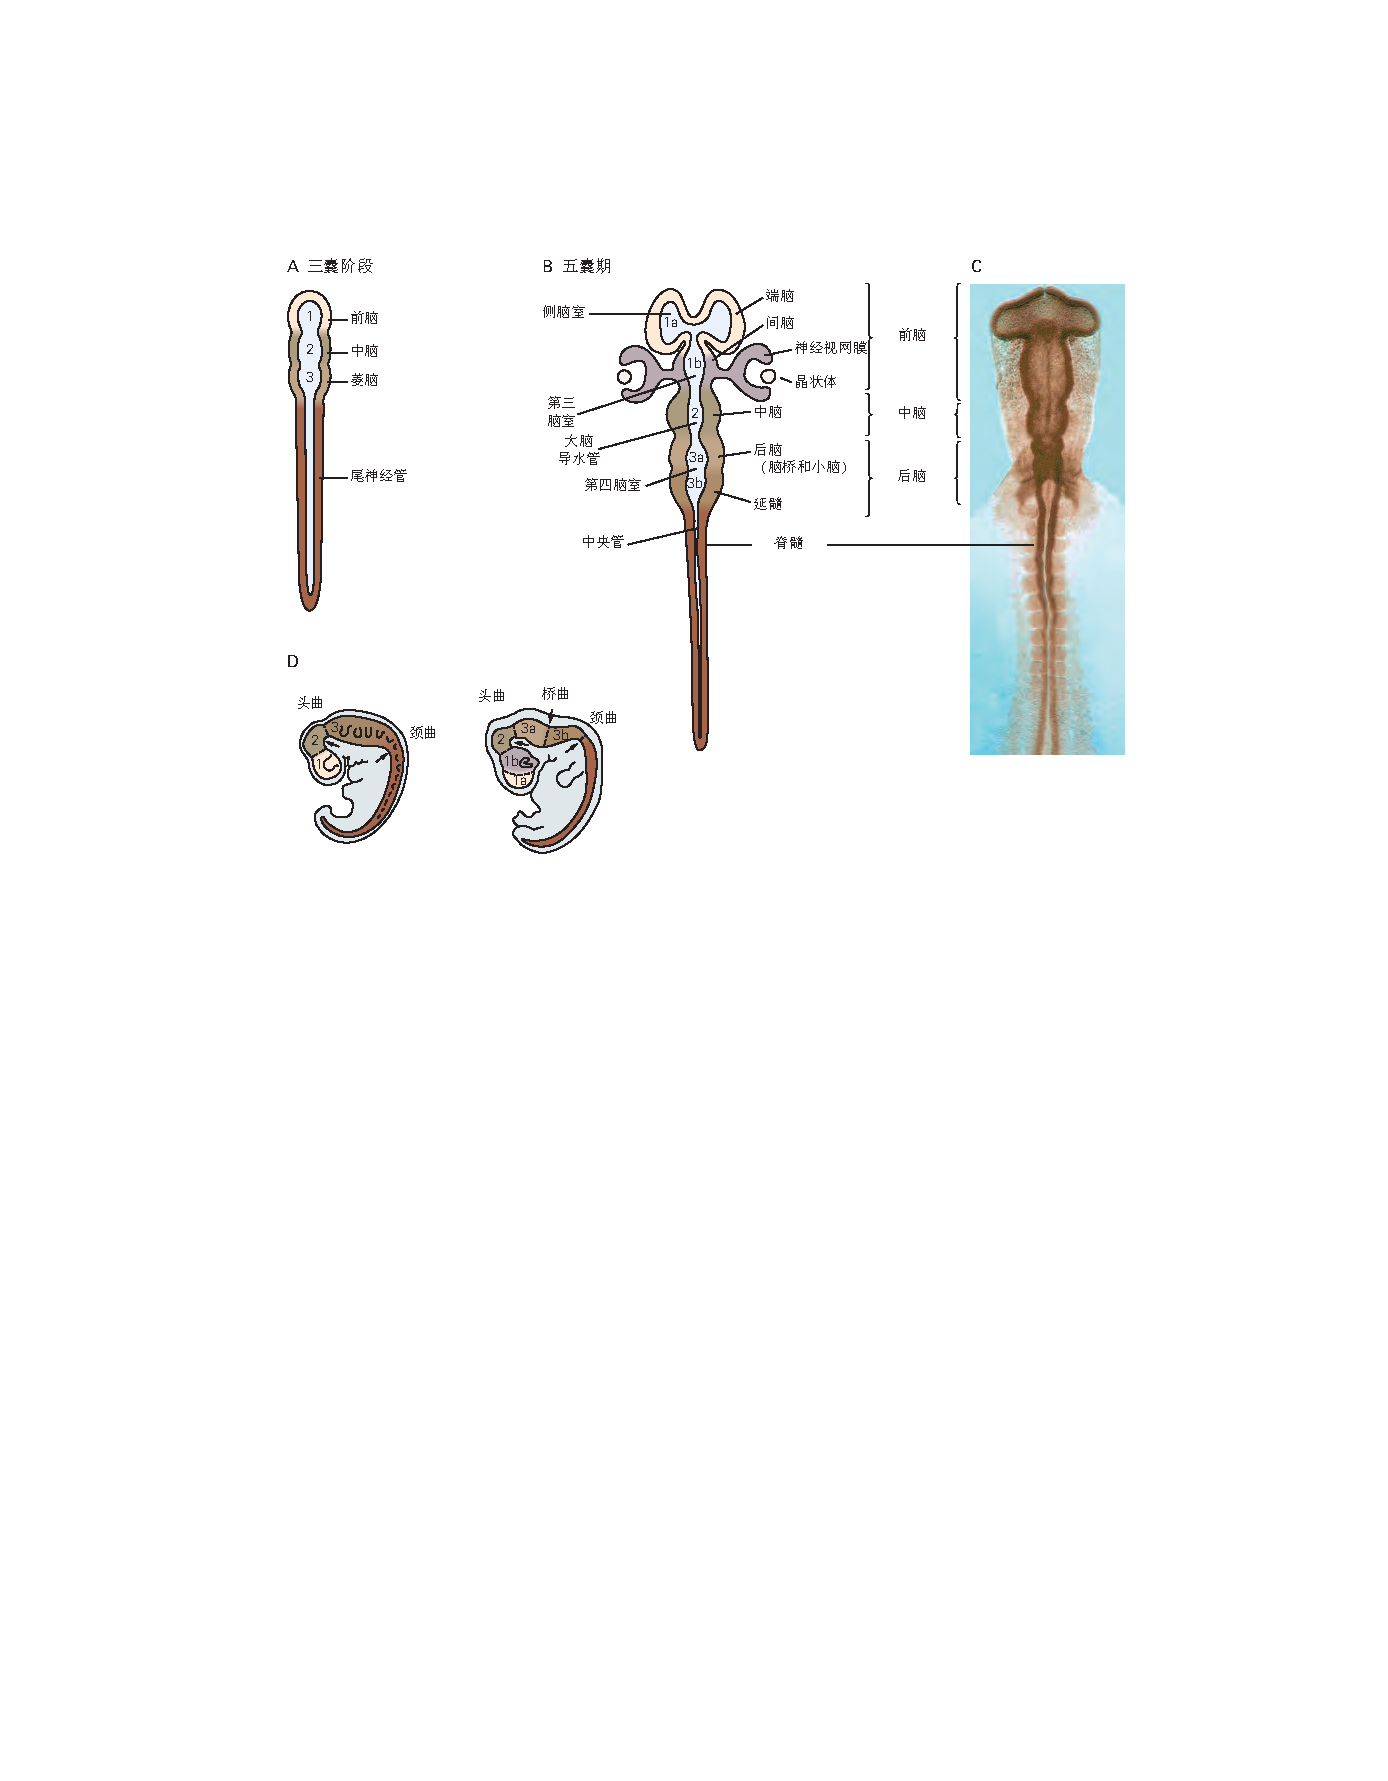
\includegraphics[width=0.8\linewidth]{chap45/fig_45_4}
	\caption{神经管发育的连续阶段。 A. 在神经管发育的早期阶段,有三个脑泡,它们将形成前脑(前脑)、中脑(中脑)和菱脑(后脑)。 B. 前脑和菱脑内的进一步分裂产生额外的囊泡。 前脑分裂形成端脑和间脑,菱脑分裂形成后脑和髓脑。 C. 五囊泡阶段鸡胚神经管的俯视图。 (经许可转载自 G. Schoenwolf。) D. 神经管在小泡之间的边界处弯曲,形成头曲、脑桥曲和颈曲。}
	\label{fig:45_4}
\end{figure}


在这个早期的三囊泡阶段,神经管弯曲两次:一次在颈曲处,在脊髓和后脑的交界处,一次在头曲处,在后脑和中脑的交界处。
第三个弯曲,桥脑弯曲,形成较晚,更晚,颈椎弯曲变直并变得模糊(图 \ref{fig:45_4}D)。 头曲在整个发育过程中保持突出,它的持续存在是前脑纵轴方向偏离脑干和脊髓方向的原因。

随着神经管的发育,两个初级胚胎小泡进一步分裂,从而形成五个小泡(图 45–4B、C)。 前脑囊泡分裂形成端脑,端脑会产生皮质、海马和基底神经节,间脑会产生丘脑、下丘脑和视网膜。 中脑不再进一步分裂,产生下丘和上丘以及其他中脑结构。 后脑囊泡分裂形成后脑,后脑会产生脑桥和小脑,以及中脑,后脑会产生延髓。 这些部分与脊髓一起构成了成熟中枢神经系统的主要功能区域(见第 \ref{chap:chap4} 章)。 神经管逐渐细分为这些功能域受各种分泌信号的调节。

\subsection{来自中胚层和内胚层的信号定义了神经板的 Rostrocaudal 模式}
最初认为,按照 Spemann 和 Mangold 的定义,组织者的特征是一致的,因此诱导了最初一致的神经板。 然而,随后的研究表明,组织者是区域性的,并且几乎在感应开始时就分泌启动神经板 rostrocaudal 模式的因子。 一类重要的因子包括 Wnt 蛋白(基于其创始家族成员的首字母缩写词,果蝇 Wingless 蛋白和哺乳动物 Int1 原癌基因蛋白)。 其他包括视黄酸和 FGF。 它们由组织者的中胚层细胞以及附近的近轴中胚层产生。

Wnt 信号活动的净水平在神经板的吻端水平较低,并在尾端方向逐渐增加。 这种活动梯度的出现是因为与神经板尾部区域相邻的中胚层表达高水平的 Wnt。 神经板延髓区域下方的组织加强了这种梯度,是抑制 Wnt 信号的分泌蛋白的来源,就像 BMP 抑制剂在早期阶段减弱 BMP 信号一样。 
因此,沿着神经板在越来越多的尾部位置的细胞暴露于不断增加的 Wnt 活性水平,并获得更多的尾部区域特征,跨越从前脑到中脑再到后脑最后到脊髓的整个范围(图 \ref{fig:45_5}A)。 
这些结果表明,前部特征是神经组织的“默认”状态,Wnt 等信号强加了后部特征。 实际上,当通过应用 BMP 抑制剂诱导外胚层细胞成为神经细胞时,它们会分化为具有前部结构特征的细胞。

\begin{figure}[htbp]
	\centering
	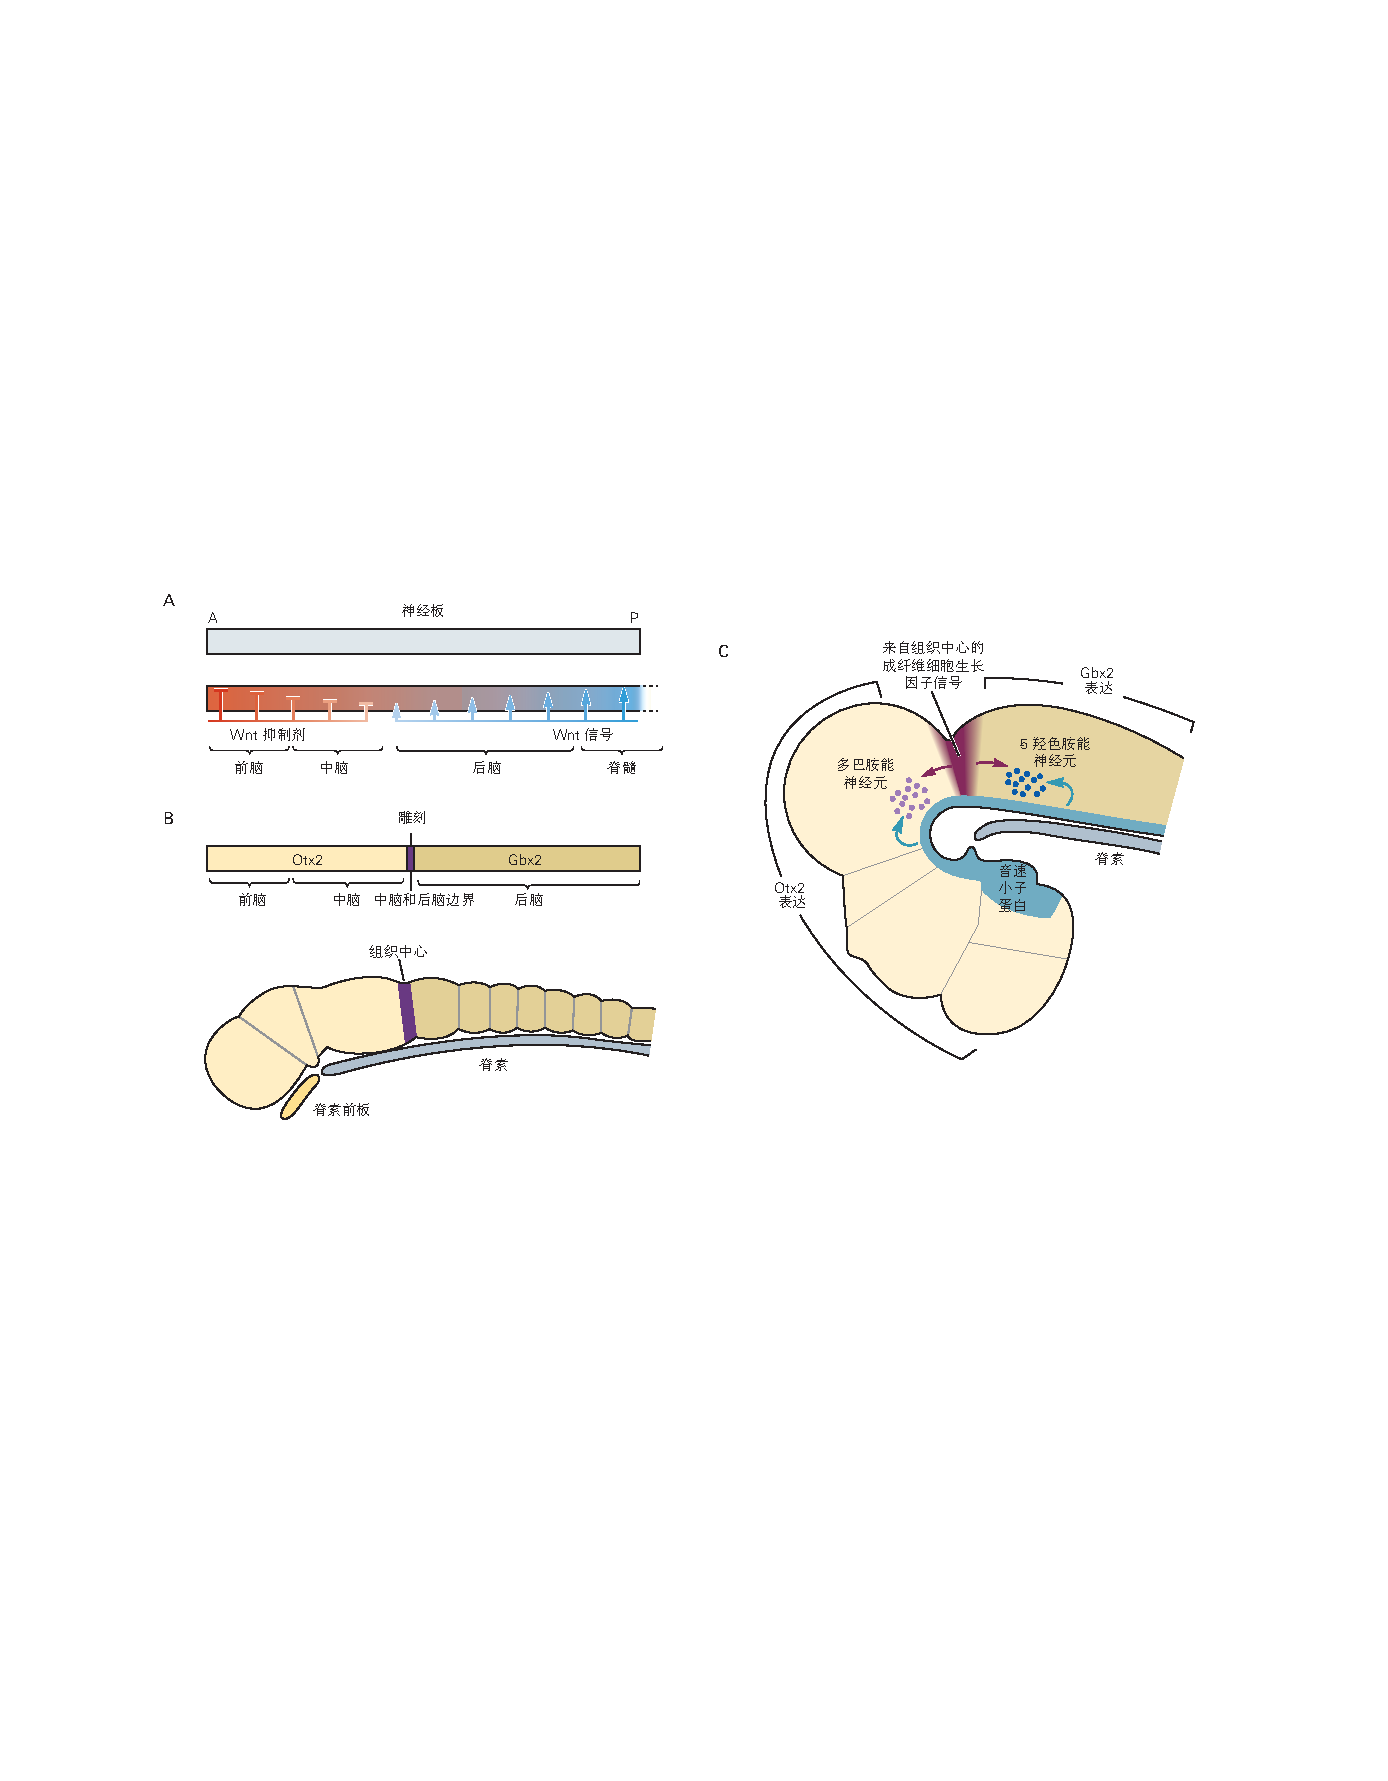
\includegraphics[width=0.5\linewidth]{chap45/fig_45_5}
	\caption{早期前后模式信号建立不同的转录因子域并定义中脑-后脑边界区域的位置。 A. 神经板的前后模式是通过将神经细胞暴露于 Wnt 信号梯度来建立的。 神经板的前 (A) 区域暴露于内胚层分泌的 Wnt 抑制剂,因此仅感知低水平的 Wnt 活性。 神经板的更多后 (P) 区域逐渐暴露于来自近轴中胚层的高水平 Wnt 信号和较低水平的 Wnt 抑制剂。 B. 为了响应此 Wnt 信号梯度和其他信号,神经板前部和后部区域的细胞开始表达不同的转录因子:前部水平的 Otx2 和更后部水平的 Gbx2。 这两个转录因子结构域的交叉点标志着中脑-后脑边界 (MHB) 区域,其中表达了 Engrailed 转录因子。 然后神经管形成 MHB 前后的部分。 C. 来自峡部组织者的成纤维细胞生长因子 (FGF) 信号与来自腹侧中线的声波刺猬 (Shh) 信号协同作用,以指定多巴胺能和血清素能神经元的身份和位置。 这两类神经元的不同命运源于 Otx2 在中脑和 Gbx2 在后脑中的表达。 (经许可改编自 Wurst 和 Bally-Cuif 2001。版权所有 © 2001 Springer Nature。)}
	\label{fig:45_5}
\end{figure}

\subsection{来自神经管内组织中心的信号会影响前脑、中脑和后脑}
中胚层和内胚层组织对 rostrocaudal 神经模式的早期影响通过来自神经管本身的特殊细胞群的信号进一步完善。 一个已经被特别详细研究过的被称为峡部组织器,它形成在后脑和中脑的边界处(图 \ref{fig:45_5}B)。 峡部组织者在神经管的这两个区域的模式化以及指定其中的神经元类型方面起着关键作用。 黑质和腹侧被盖区的多巴胺能神经元在中脑中产生,就在峡部组织者的头端,而中缝核的血清素能神经元在后脑内在峡部组织者的尾部产生。 为了说明这些二级神经信号中心如何施加神经模式,我们描述了峡部组织者的起源和信号活动。

神经板的 rostrocaudal 位置特征源于同源域转录因子的表达,同源域是蛋白质的一部分,它与基因调节区域中的特定 DNA 序列结合,导致基因转录发生变化。 神经板前脑和中脑区域的细胞表达 Otx2,而后脑区域的细胞表达 Gbx2,两者都是同源域转录因子。 Otx2 和 Gbx2 表达之间的转换点位于中脑-后脑边界(图 \ref{fig:45_5}B),标志着神经管闭合后峡部组织者出现的位置。 在此边界处,表达了其他转录因子,特别是 En1(一种 Engrailed 类转录因子)。

这些转录因子反过来控制峡部组织细胞的两个信号因子 Wnt1 和 FGF8 的表达。 Wnt1 参与中脑-后脑域细胞的增殖和 FGF8 表达的维持。 FGF8 从峡部组织器扩散到以 Otx2 表达为标志的中脑区域诱导多巴胺能神经元分化,而其扩散到以 Gbx2 表达为标志的后脑区域触发血清素能神经元的分化(图 \ref{fig:45_5}C)。

FGF8 和 Wnt1 在来自峡部组织者的信号中的作用说明了早期神经模式的重要经济性。 感应信号的早期作用强加了转录因子表达的离散域,然后这些转录域允许细胞以不同方式解释同一分泌因子的作用,从而产生不同的神经元亚型。 通过这种方式,相对少量的分泌因子——FGF、BMP、刺猬蛋白、Wnt 蛋白和视黄酸——被用于不同区域和不同时间,以对中枢和外周神经细胞内产生的大量神经元细胞类型进行编程 神经系统。

其他细胞群在将神经管细分为多个域方面起着类似的作用。 例如,在神经管的最前端边缘,有一组特殊的细胞,称为前神经嵴,分泌 FGF,形成端脑(图 45-6)。 
更靠近尾部的是一个限制区域,称为 zona limitans intrathalamica,它在间脑内表现为一对角状骨刺。 Zona limitans intrathalamica 细胞分泌蛋白 sonic hedgehog (Shh),它会在附近的细胞中形成图案,从而产生丘脑的细胞核。 FGF 和 Shh 分别在它们在皮质和脊髓模式化中的突出作用的背景下进行了详细描述。

\begin{figure}[htbp]
	\centering
	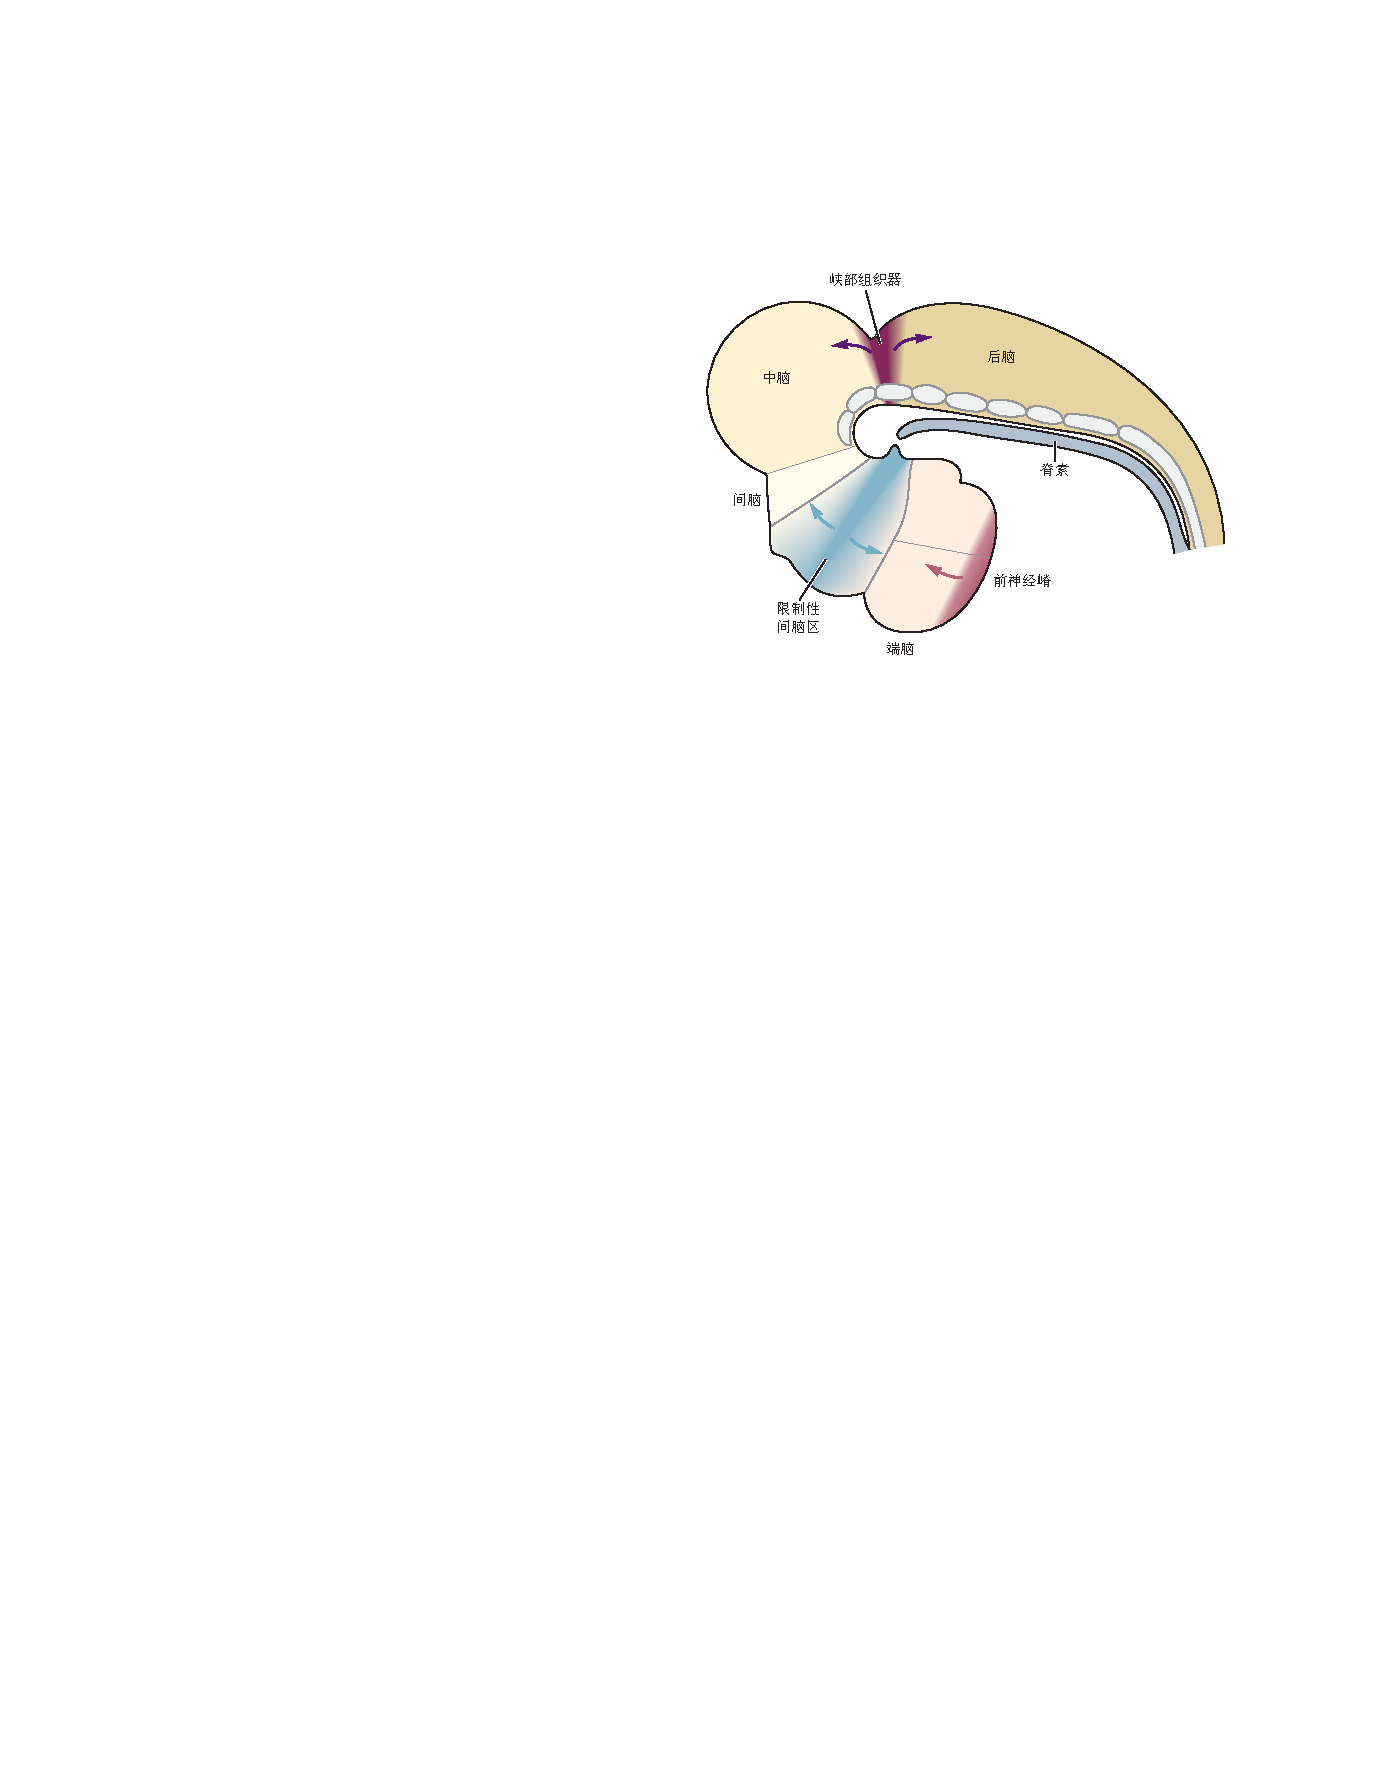
\includegraphics[width=0.6\linewidth]{chap45/fig_45_6}
	\caption{发育中的神经管中的局部信号中心。 这张神经管后期的侧视图显示了三个关键信号中心的位置,这些信号中心沿着前后轴排列神经管:前神经嵴、位于头侧和侧侧边界的丘脑内限制带 (ZLI) 尾部前脑(间脑)和峡部组织者,中脑和后脑的边界。 ZLI 是声波刺猬的来源,峡部组织者和前神经嵴是成纤维细胞生长因子的来源(见图 45-5)。}
	\label{fig:45_6}
\end{figure}

\subsection{抑制性相互作用将后脑分成几个部分}

沿 rostrocaudal 轴排列神经管的重要下一步是将前脑和后脑细分为段,即沿 rostrocaudal 轴排列的隔室单元。 这些单位在前脑中称为前体,在后脑中称为菱形体。

我们使用菱形节 3 和 4(共 7 个)的形成来说明导致分割的机制(图 \ref{fig:45_7})。 
初始形态发生素梯度导致该区域表达两种不同的转录因子——krox20 在将成为菱形节 3 的区域中,赋予这些细胞以菱形节 3 身份,而 hoxb1 在将成为菱形节 4 的区域中,赋予这些细胞以菱形节 4 身份 . 边界附近的细胞表达这两种因素,因此具有不确定的身份。 然而,这两个因素相互抑制对方的表达,所以最终每个细胞的身份都是固定的。

\begin{figure}[htbp]
	\centering
	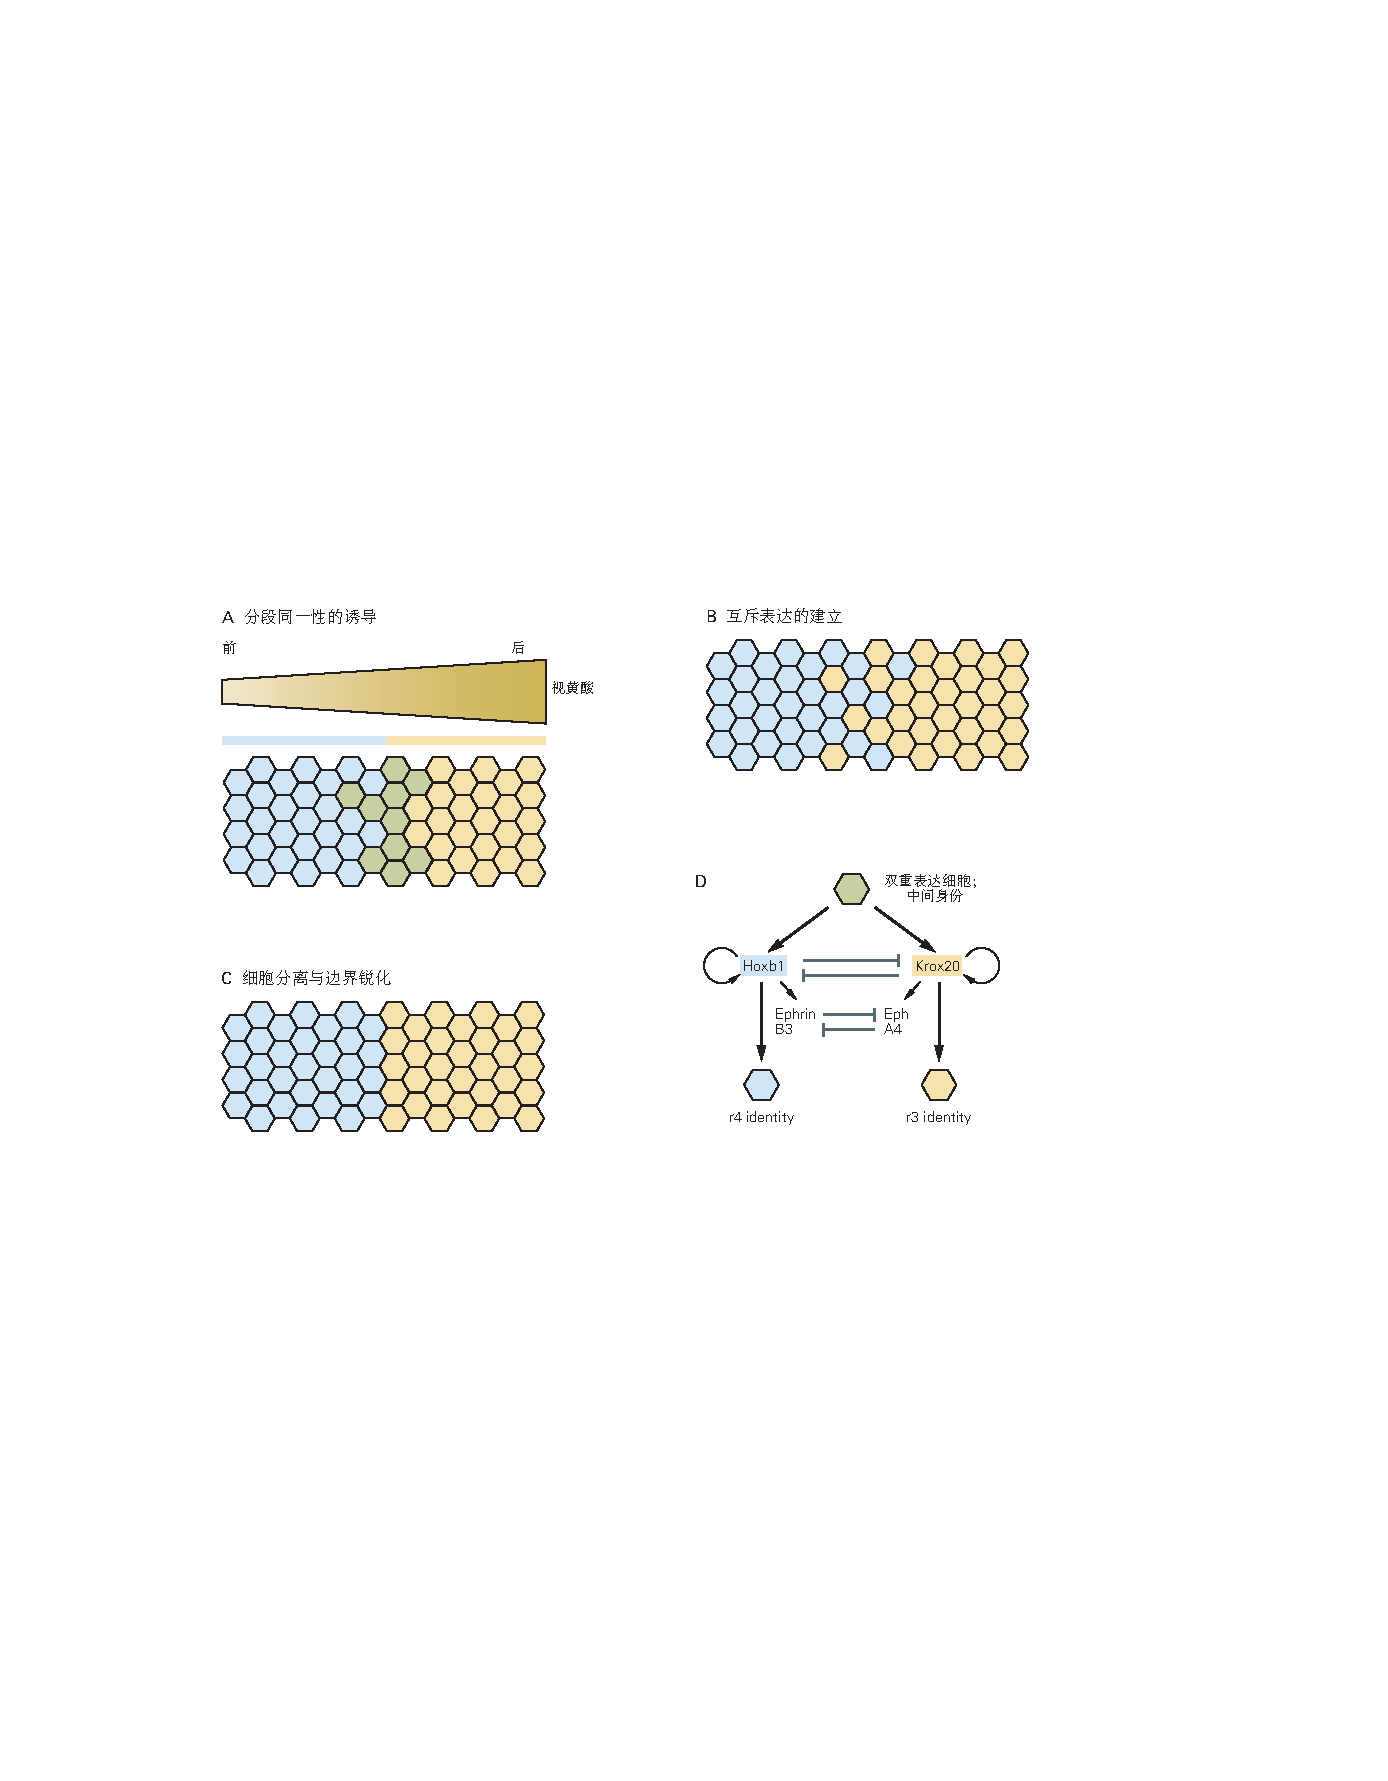
\includegraphics[width=0.5\linewidth]{chap45/fig_45_7}
	\caption{抑制性相互作用将后脑分成菱形节。 后脑 rhombomeres 3 和 4 之间的锐利边界分几个步骤形成。 (经许可改编自 Addison 和 Wilkinson,2016 年。版权所有 © 2016 Elsevier Inc.) 表达两个基因的预期边界(绿色)。 B. Hoxb1 表达和 Krox20 表达变得相互排斥,从而赋予每个细胞独特的分子身份。 C. 被困在错误域中的细胞迁移以锐化边界。 D. 边界形成的抑制性相互作用。 Hoxb1 和 Krox20 在单个细胞中相互抑制彼此的表达,因此水平的适度不平衡会导致一个因子的独占表达。 然后 Krox20 在 r3 细胞中上调 EphA4,而在 r4 细胞中上调 ephrinB3。 EphA4 和 ephrinB3 相互排斥,驱动分离细胞的迁移并锐化片段边界。}
	\label{fig:45_7}
\end{figure}

问题是一些细胞被困在了错误的菱形节内。 这种混合可以通过多种方式纠正,其中一种是第二种抑制相互作用,这是一种明显不同的类型。 Krox20 和 Hoxb1 分别诱导称为 EphA4 和 ephrinB3 的细胞表面识别和信号分子的表达。 这两种蛋白质相互结合,导致分离细胞的排斥信号的传输。 我们将在下面看到,这种排斥力也是轴突在向目标生长时做出的后期决定的关键。 在后脑中,在神经元形成之前,它会锐化菱形节之间的边界。 更广泛地说,菱形节分离提供了神经发育中普遍主题的另一个例子:诱导或粘附相互作用与抑制或抑制相互作用相结合,形成神经系统模式。

\section{神经管的背腹模式在不同的尾部水平涉及相似的机制}
随着神经上皮细胞获得其 rostrocaudal 特征,位于其背腹轴不同位置的细胞也开始获得不同的身份。 一起,沿着 rostrocaudal 和 dorsoventral 轴的图案将神经管分成分子不同的细胞类型的三维网格,最终导致产生将神经系统的一部分与另一部分区分开来的各种神经元和神经胶质细胞类型。

与负责发育神经元头尾模式的信号和组织中心的多样性相反,建立背腹模式的策略和原则具有惊人的一致性。 我们最初专注于产生脊髓的神经管尾端背腹模式的机制,然后描述如何使用类似的策略来模式化前脑。

脊髓中的神经元有两个主要功能。 它们将皮肤感觉输入中继到大脑的更高中枢,并将感觉输入转化为运动输出。 介导这些功能的神经回路在解剖学上是分离的。 涉及处理皮肤感觉信息的电路位于脊髓的背侧半部,而涉及运动输出控制的电路主要位于脊髓的腹侧半部。

形成这些回路的神经元是在从不同祖细胞类型的建立开始的模式化过程中沿着脊髓背腹轴的不同位置产生的。 运动神经元在腹侧中线附近产生,并且大多数控制运动输出的中间神经元类在运动神经元出现的位置的背侧产生(图 \ref{fig:45_8})。 
神经管的后半部分产生投射神经元和处理传入感觉信息的局部回路中间神经元。

\begin{figure}[htbp]
	\centering
	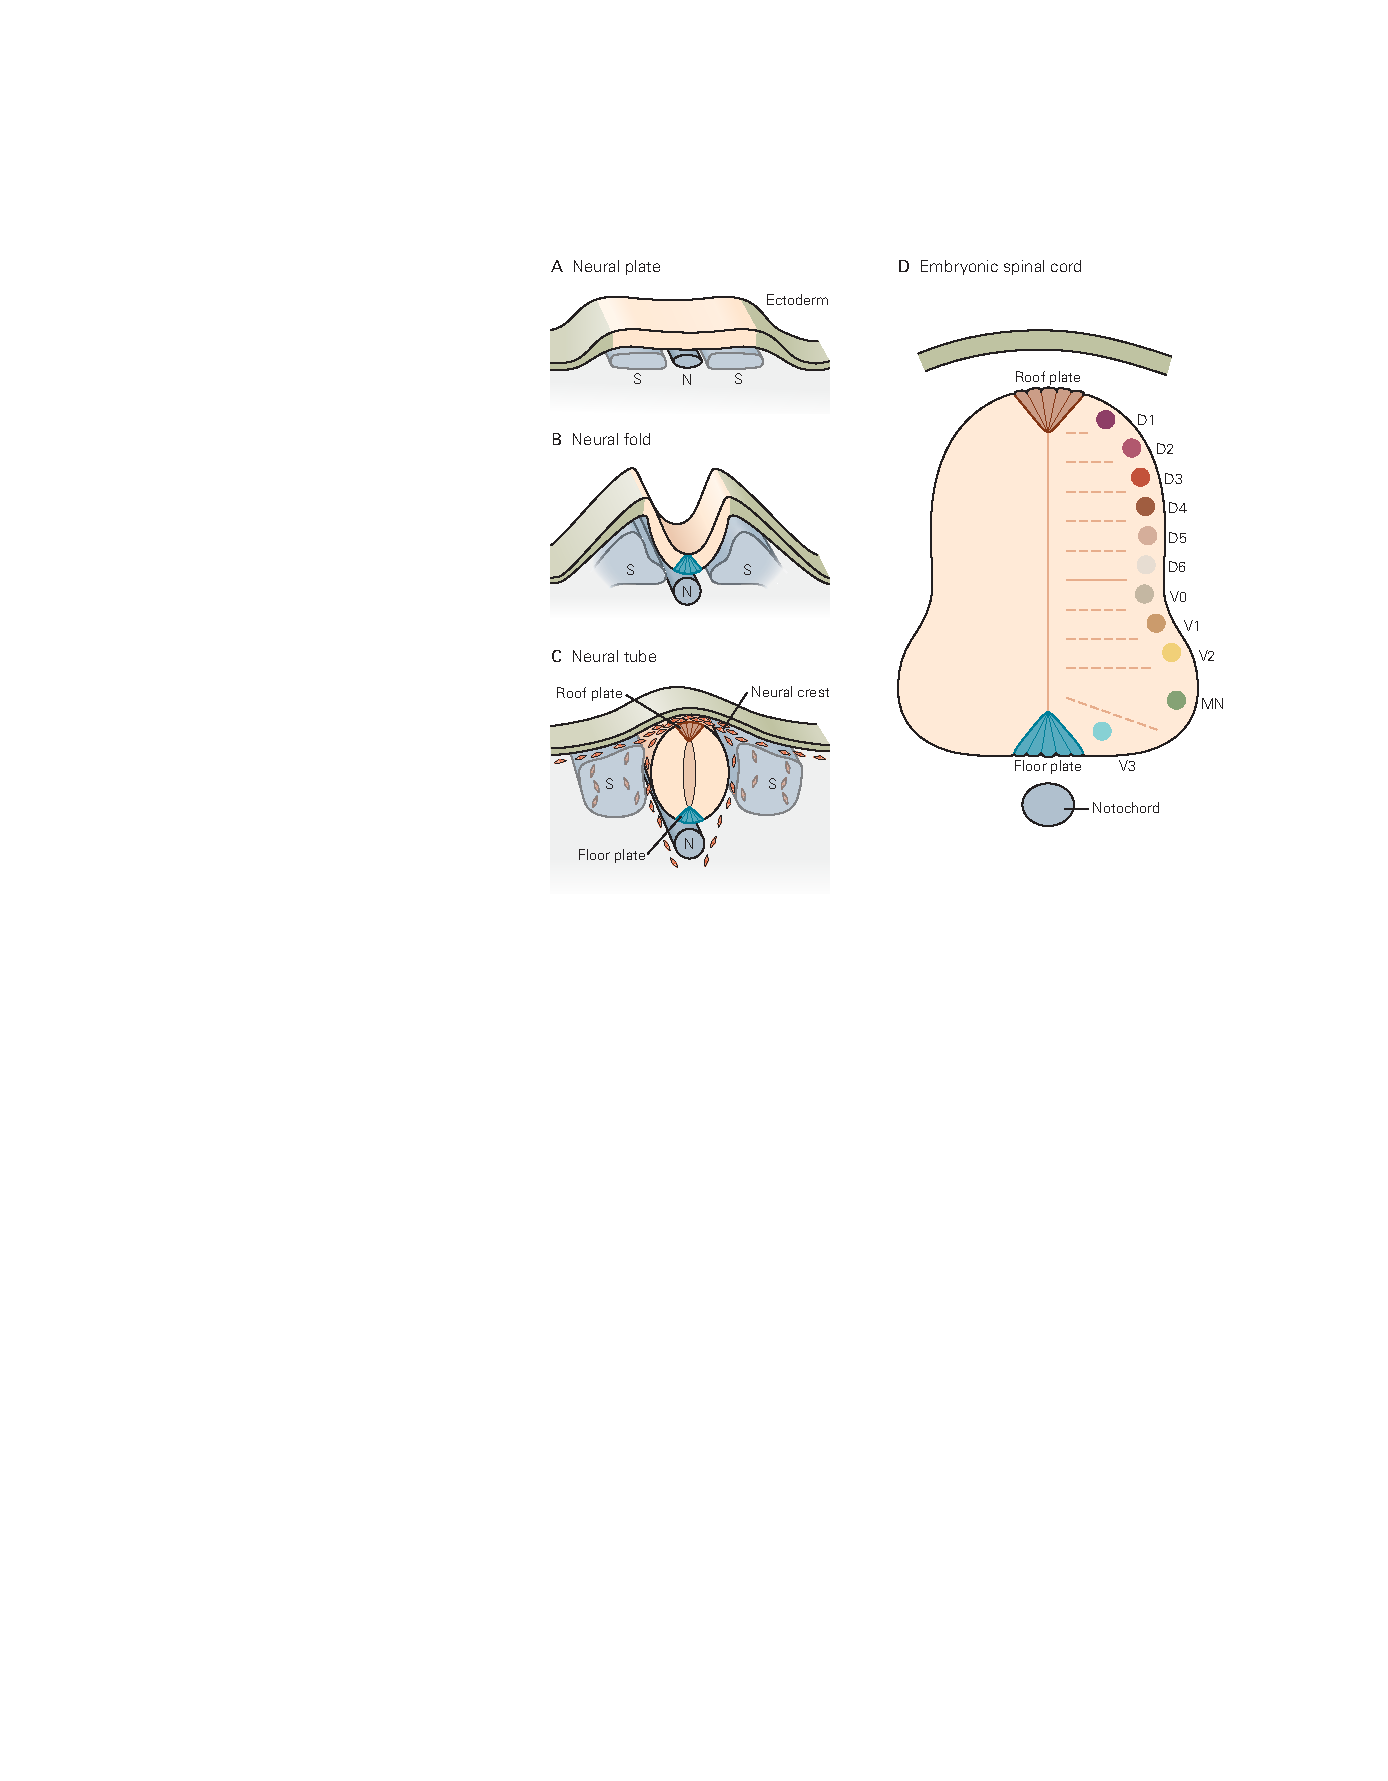
\includegraphics[width=0.7\linewidth]{chap45/fig_45_8}
	\caption{不同的前体种群沿着发育中的脊髓的背腹轴形成。 A. 神经板由覆盖脊索 (N) 和未来体节 (S) 的外胚层细胞生成。 它的两侧是表皮外胚层。 (另请参见图 45-1) B. 神经板在其中线处向背面折叠,形成神经褶皱。 底板细胞(蓝色)在神经管的腹侧中线处分化。 C. 神经管通过神经皱襞的背尖融合形成。 屋顶板细胞在神经管的背侧中线形成。 在填充感觉和交感神经节之前,神经嵴细胞从神经管迁移到并经过体节。 D. 不同类别的神经元在胚胎脊髓的不同背腹位置产生。 腹侧中间神经元 (V0–V3) 和运动神经元 (MN) 与腹侧脊髓中的祖细胞域不同。 六类早期背侧中间神经元 (D1–D6) 在脊髓的背侧半部发育。 (改编自 Goulding 等人,2002 年。)}
	\label{fig:45_8}
\end{figure}

脊髓神经元的位置和身份是如何确定的? 神经管的背腹模式由靠近神经管腹侧和背极的中胚层和外胚层细胞发出的信号启动,并由两个中线神经组织中心发出的信号延续。 腹侧图案化信号最初由脊索提供,脊索是位于腹侧神经管正下方的中胚层细胞群(图 \ref{fig:45_1})。 这种信号活动被转移到底板,这是一个专门的神经胶质细胞群,位于神经管本身的腹侧中线。 同样,背侧信号最初由跨越神经管背侧中线的表皮外胚层细胞提供,随后由顶板提供,屋顶板是嵌入神经管背侧中线的神经胶质细胞群(图 \ref{fig:45_8})。

因此,神经模式是通过同源诱导过程启动的,在这个过程中,同类产生类似的结果:脊索信号诱导底板,诱导腹侧神经元,来自外胚层的信号诱导顶板,诱导背侧神经元。 随着组织生长和细胞移动,该策略确保感应信号被适当定位以控制神经细胞在长期发育过程中的命运和模式。

\subsection{腹侧神经管由脊索和底板分泌的 Sonic Hedgehog 蛋白形成图案}
在神经管的腹侧一半内,发育中的运动神经元和局部中间神经元的身份和位置取决于 Shh 蛋白的诱导活性,该蛋白由脊索分泌,随后由底板分泌。 Shh 是与 Drosophila hedgehog 蛋白相关的分泌蛋白家族的成员,该蛋白较早被发现并显示可控制胚胎发育的许多方面。

Shh 信号对于诱导在脊髓腹侧半部产生的每个神经元类别是必需的。 单个感应信号如何指定至少六个神经元类别的命运? 答案在于 Shh 充当形态发生素的能力——一种可以在不同浓度阈值下指导不同细胞命运的信号。 Shh 从脊索和底板的分泌在腹侧神经管中建立了一个从腹侧到背侧的 Shh 蛋白活性梯度,使得在神经上皮细胞内占据不同背腹侧位置的祖细胞暴露于小的(2 到 3 个) fold) 环境 Shh 信号活动的差异。 
不同水平的 Shh 信号活动指导不同腹侧区域的祖细胞分化为运动神经元和中间神经元(图 \ref{fig:45_9}A)。

\begin{figure}[htbp]
	\centering
	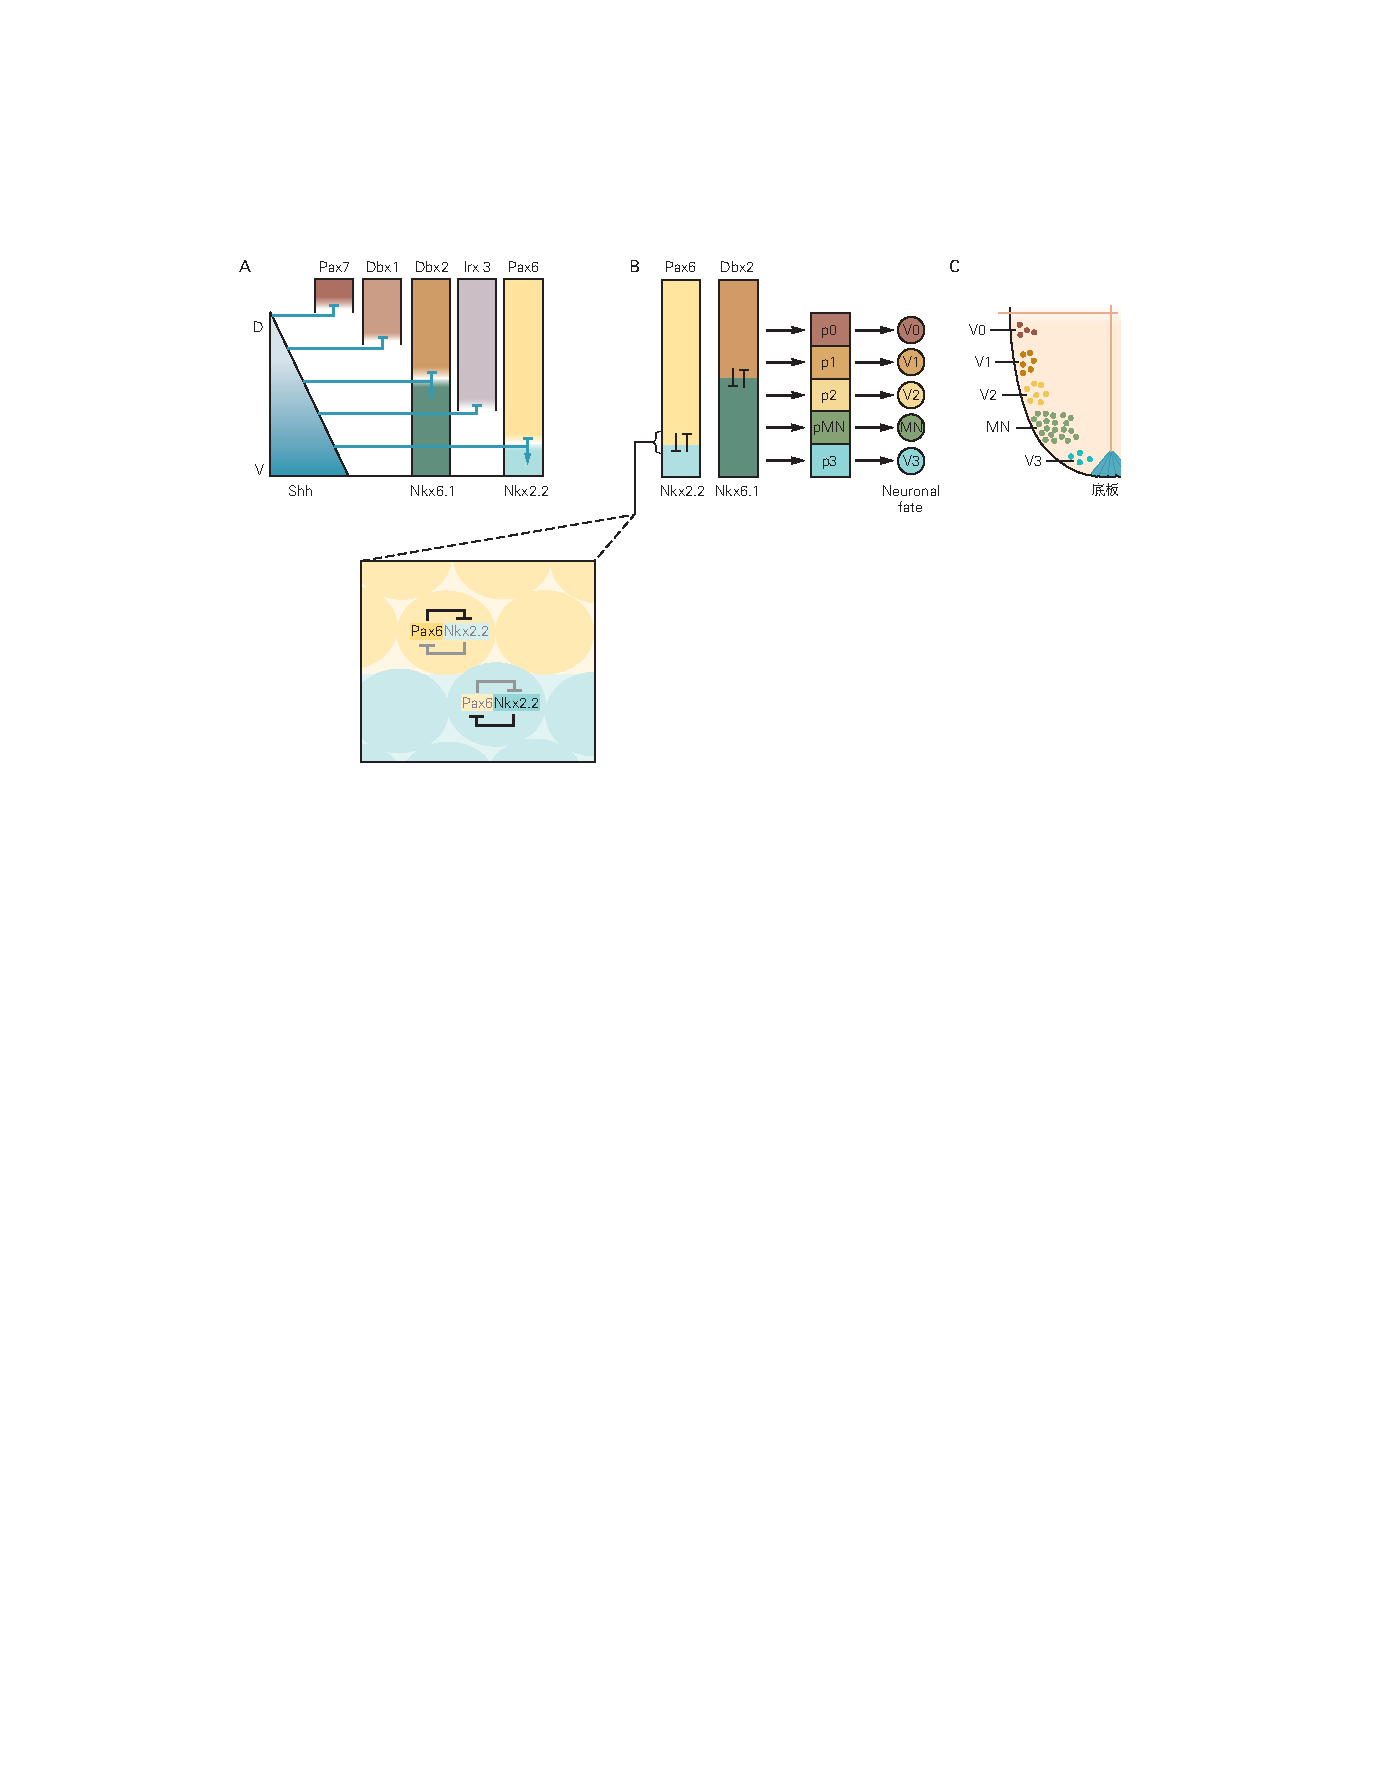
\includegraphics[width=0.8\linewidth]{chap45/fig_45_9}
	\caption{声波刺猬信号梯度控制腹侧脊髓中的神经元特性和模式。 A. 声波刺猬 (Shh) 信号的腹侧到背侧 (V–D) 梯度在神经管腹侧一半内的祖细胞中建立同源域蛋白表达的背腹域。 在每个浓度下,不同的同源域转录因子(Pax7、Dbx1、Dbx2、Irx3 或 Pax6)受到抑制,其中 Pax7 最敏感,Pax6 对抑制最不敏感。 其他同源域转录因子(Nkx6.1 和 Nkx2.2)在不同的 Shh 水平上被诱导。 邻接共同祖域边界的同源域蛋白具有相似的 Shh 抑制和激活浓度阈值。 分级的 Shh 信号产生相应的 Gli 转录因子活性梯度(未显示)。 B. Shh/Gli 信号诱导或抑制的转录因子之间的交叉抑制指定了不同的神经元类别。 例如,Pax6 和 Nkx2.2,以及 Dbx2 和 Nkx6.1,以细胞自主方式起作用以抑制彼此的表达(插图),以明确的方式将细胞身份赋予祖细胞。 分级 Shh 和 Gli 信号的顺序影响,连同同源结构域转录交叉抑制,建立了五个主要的祖细胞结构域。 C. 从这些域中出现的有丝分裂后神经元产生五个主要类别的腹侧神经元:中间神经元 V0–V3 和运动神经元 (MN)。}
	\label{fig:45_9}
\end{figure}

这些发现提出了另外两个问题。 Shh 蛋白在腹侧神经上皮细胞内的扩散是如何以如此精确的方式控制的? Shh 信号活动的微小差异如何转化为关于腹侧神经管中祖细胞身份的全有或全无决定?

活性 Shh 蛋白由较大的前体蛋白合成,通过不寻常的自催化过程裂解,该过程涉及驻留在前体蛋白羧基末端的丝氨酸蛋白酶样活性。 切割产生一个氨基末端蛋白片段,该片段具有 Shh 的所有信号传导活性。 在切割过程中,通过添加胆固醇分子共价修饰活性氨基末端片段。 在 Shh 分泌后,这种亲脂性锚将大部分蛋白质束缚在脊索和底板细胞的表面。 然而,一小部分锚定蛋白从细胞表面释放,并在腹侧神经上皮细胞内从一个细胞转移到另一个细胞。 实际上,确保形成细胞外 Shh 蛋白长距离梯度的分子机制更为复杂,涉及促进 Shh 从底板释放的特殊跨膜蛋白,以及调节 Shh 蛋白在细胞间转移的蛋白质。

腹侧神经管内 Shh 蛋白的梯度如何沿着不同的分化途径引导祖细胞? Shh 信号通过它与跨膜受体复合物的相互作用而启动,该复合物由称为 patched 的配体结合亚基和称为 smoothened 的信号转导亚基(以相应的果蝇基因命名)组成。 Shh 与 patched 的结合解除了它对 smoothened 的抑制作用,因此激活了一种涉及多种蛋白激酶、转运蛋白和最重要的 Gli 蛋白(一类锌指转录因子)的细胞内信号通路。

在没有 Shh 的情况下,Gli 蛋白被蛋白水解加工成转录抑制因子,从而阻止 Shh 靶基因的激活。 Shh 信号通路的激活会抑制这种蛋白水解过程,结果是 Gli 的转录激活因子形式占主导地位,从而指导 Shh 靶基因的表达。 以这种方式,Shh 蛋白的细胞外梯度被转化为 Gli 激活蛋白的核梯度。 Gli 抑制蛋白和激活蛋白在不同背腹位置的比例决定了哪些靶基因被激活。

Shh-Gli 信号激活了哪些基因,它们如何参与腹侧神经元亚型的规范化? Gli 的主要目标是编码更多转录因子的基因。 一类主要的 Gli 目标编码同源域蛋白,转录因子包含称为同源盒的保守 DNA 结合基序。 第二大类目标基因编码具有基本螺旋环-螺旋 DNA 结合基序的蛋白质。 一些同源结构域和基本螺旋-环-螺旋蛋白被抑制,而另一些被 Shh 信号激活,每个都处于特定的浓度阈值。 通过这种方式,腹侧神经管中的细胞被分配到五个主要祖细胞域之一,每个域都有自己的转录因子谱(图 \ref{fig:45_9}B,C)。

定义相邻祖细胞结构域的转录因子会抑制彼此的表达。 因此,尽管一个细胞最初可能表达几种转录因子,这些转录因子可以指导细胞沿不同的分化途径,但两种因子起始浓度的轻微不平衡会通过抑制迅速放大,并且只有一种蛋白质稳定表达。 这种转录抑制的赢者通吃策略锐化了祖细胞域的边界,并确保 Shh 和 Gli 活性的初始梯度将自身分解为转录因子谱中的明显区别。 指定腹侧祖细胞结构域的转录因子然后指导下游基因的表达,这些基因将祖细胞提交给特定的有丝分裂后神经元身份。 因此,对 Shh 信号的研究不仅揭示了腹侧神经元模式化的逻辑,而且还证明了神经元的命运部分取决于转录抑制因子而非激活因子的作用。 这一原则适用于许多其他组织和生物体。

尽管最初是在神经发育的背景下进行研究,但 Shh 信号的缺陷现在与多种人类疾病有关。 人类 Shh 通路基因的突变会导致腹侧前脑结构发育缺陷(前脑无裂畸形),以及脊柱裂、肢体畸形和某些癌症等神经系统缺陷。

\subsection{背神经管由骨形态发生蛋白组成}
还发现了一种基于分级形态发生素水平激活转录程序集的信号策略来确定背侧脊髓中细胞类型的模式。 神经管背侧中线顶板细胞的分化是由来自表皮细胞的 BMP 信号触发的,表皮细胞最初与神经板接壤,后来在背侧神经管两侧。

神经管关闭后,屋顶板细胞本身开始表达 BMP 和 Wnt 蛋白。 Wnt 蛋白促进背神经管中祖细胞的增殖。 BMP 蛋白诱导神经管最背侧边缘的神经嵴细胞分化,随后诱导产生不同的感觉中继神经元群,这些神经元定居在背侧脊髓中。

\subsection{背腹模式机制沿神经管的 Rostrocaudal 范围得到保护}
用于在脊髓中建立背腹模式的策略还控制沿着后脑和中脑的背腹轴以及整个前脑的大部分区域的细胞身份和模式。

在神经管的中脑区域,来自底板的 Shh 信号与前面讨论的 rostrocaudal 模式信号协同作用,以指定黑质和腹侧被盖区的多巴胺能神经元以及中缝核的血清素能神经元(见图 45) –5C). 在前脑中,来自腹侧中线的 Shh 信号和来自背侧中线的 BMP 信号共同作用以建立不同的区域域。 来自腹侧中线的 Shh 信号建立早期祖细胞域,这些区域后来产生基底神经节和一些皮质中间神经元的神经元,而来自背侧中线的 BMP 信号参与建立早期新皮质特征。


\section{局部信号决定神经元的功能子类}
至此,我们已经看到一组统一的神经前体细胞,即神经板,是如何在神经管内逐步划分为离散的头尾和背腹区域,主要是通过不同组转录调节因子的形态发生素依赖性差异表达。 下一个问题是这些域内的细胞如何继续产生神经元类型的非凡多样性,这些神经元类型是脊椎动物中枢神经系统的特征。 我们通过关注运动神经元的发育来解决这个问题。

运动神经元与中枢神经系统中所有其他类别的神经元的区别在于它们具有延伸到外周的轴突这一简单事实。 从这个角度来看,运动神经元代表了一个连贯而独特的类别。 但是运动神经元类型可以通过它们在中枢神经系统中的位置以及它们支配的靶细胞来区分。 大多数运动神经元的主要工作是支配骨骼肌,典型的哺乳动物大约有 600 块骨骼肌。 由此可知,必须有相同数量的运动神经元类型。

在本节中,我们将讨论指导这些不同功能子类分化的发育机制。 运动神经元发育的细节对于了解影响这些神经元的神经系统疾病的基础也很重要,包括脊髓性肌萎缩症和肌萎缩侧索硬化症(Lou Gehrig 病)。 在这两种疾病中,一些运动神经元类型非常脆弱,而另一些则相对有弹性。 类似的原则推动其他神经元类别多样化为不同的类型。

\subsection{头尾位置是运动神经元亚型的主要决定因素}
运动神经元沿着神经管的大部分尾轴产生,从中脑到脊髓。 
不同的运动神经元类型在每个 rostrocaudal 水平发展(图 \ref{fig:45_10}),这表明在神经管内建立 rostrocaudal 位置标识的模式信号的一个目标是使运动神经元不同。

\begin{figure}[htbp]
	\centering
	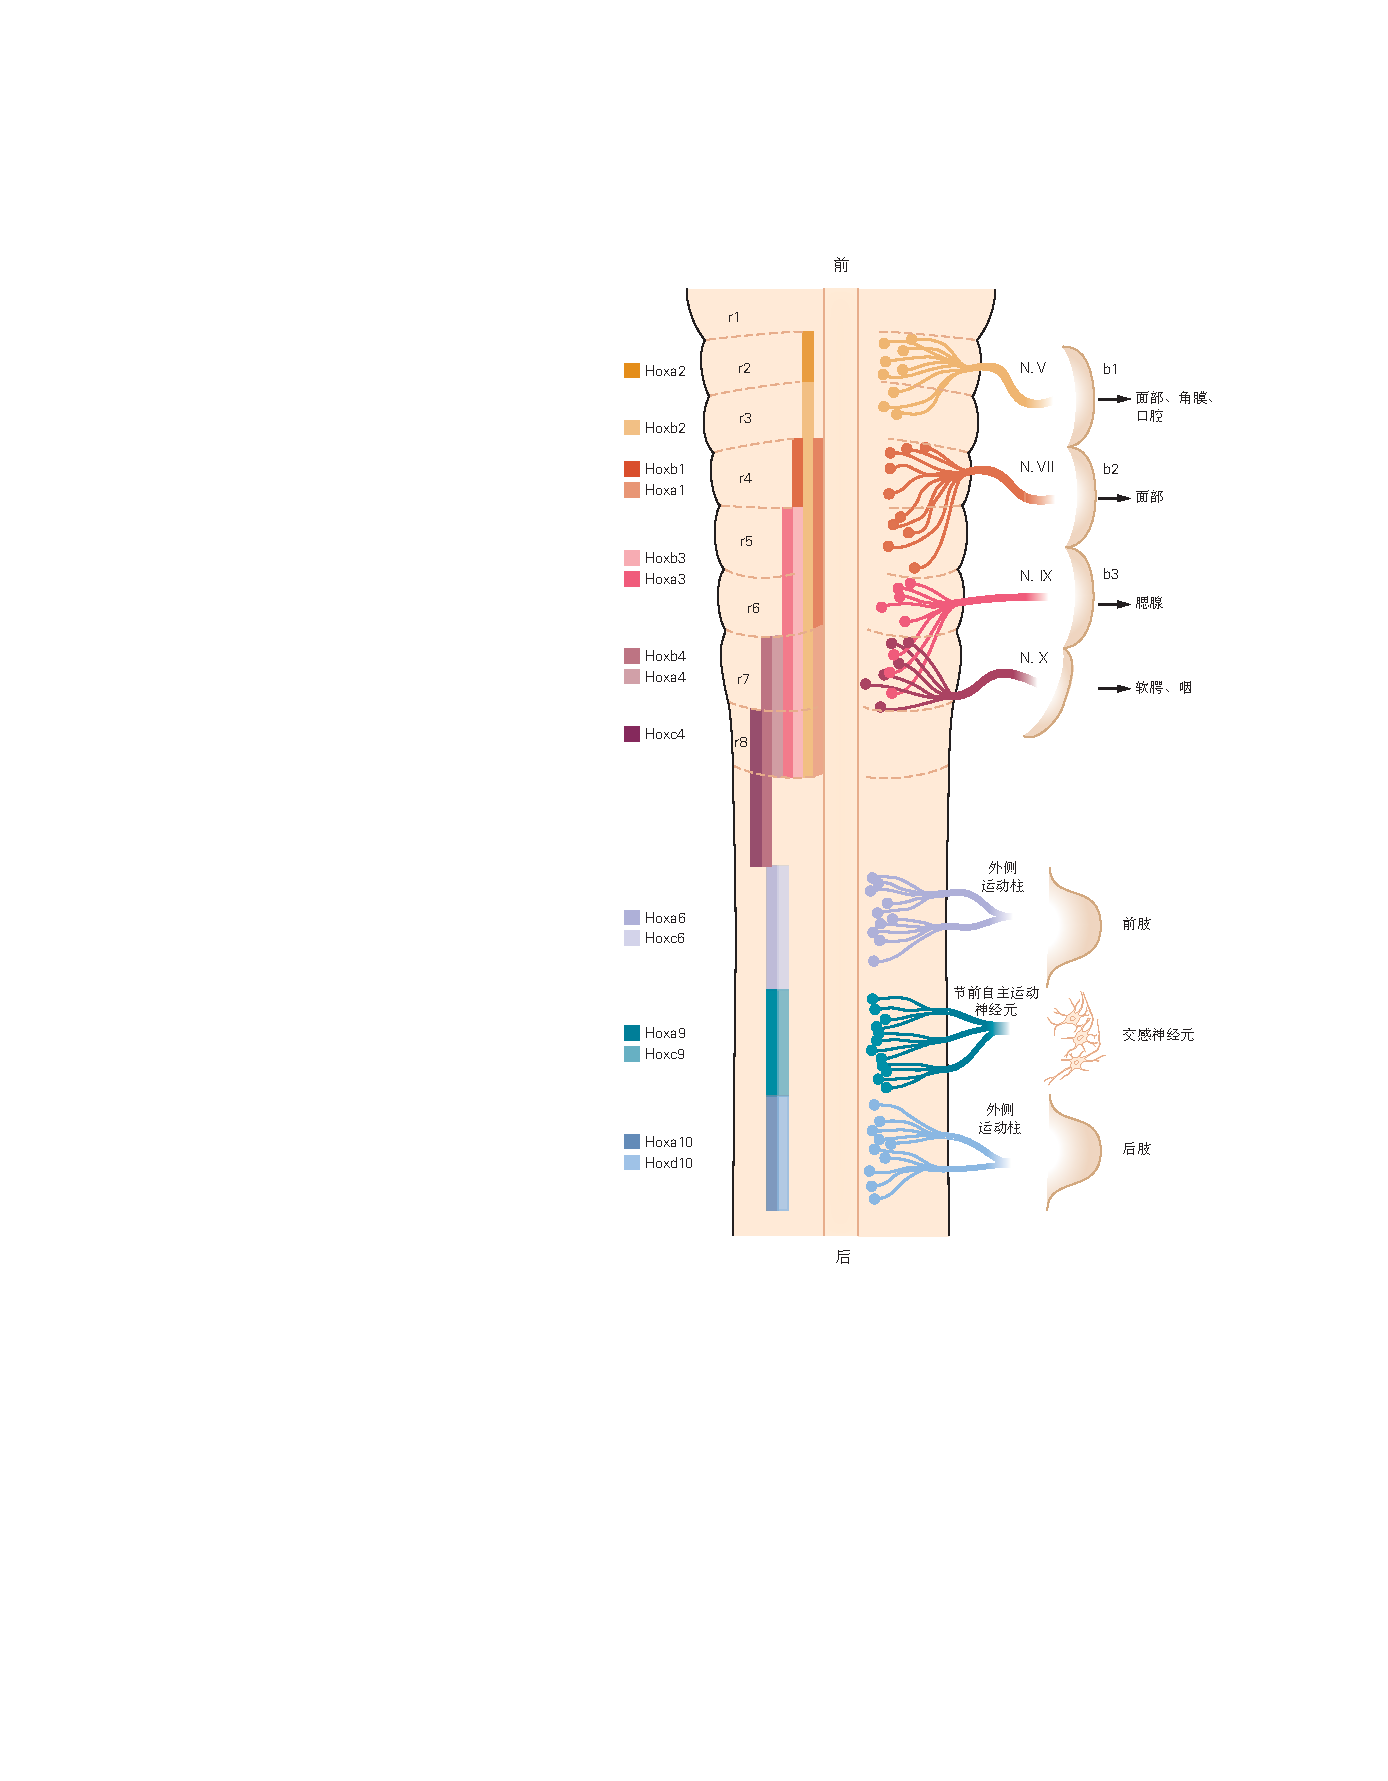
\includegraphics[width=0.65\linewidth]{chap45/fig_45_10}
	\caption{Hox 基因表达的前后分布决定了后脑和脊髓中运动神经元的亚型。 不同的 Hox 蛋白在后脑和脊髓的离散但部分重叠的 rostrocaudal 域中表达。 Hox 基因在四个哺乳动物染色体簇上的位置大致对应于它们沿神经管前后轴的表达域。 在后脑水平,运动神经元将轴突发送到颅神经 V(三叉神经)、VII(面神经)、IX(舌咽神经)和 X(迷走神经)。 这些颅运动神经投射到鳃弓 b1-b3 的外围目标。 后脑菱形节 (r1–r8) 和 Hox 配置文件显示在左侧。 在脊髓水平,将轴突发送到前肢和后肢的运动神经元包含在外侧运动柱 (LMC) 内,分别位于脊髓的肱骨和腰椎水平。 注定支配交感神经节目标的神经节前自主运动神经元 (PGC) 在胸部水平生成。 (经许可改编自 Kiecker 和 Lumsden 2005。版权所有 © 2005 Springer Nature。)}
	\label{fig:45_10}
\end{figure}

参与指定运动神经元类型的一大类基因是 Hox 基因家族。 它们的名字反映了这样一个事实,即它们是第一个发现的含有同源结构域的转录因子,同源结构域是一种 DNA 结合结构域,现在已知存在于许多转录因子中,这些转录因子调节酵母、植物和哺乳动物等多种生物体的发育过程。 例如,上面讨论的 Otx 和 Gbx 基因包含同源域。 哺乳动物的 Hox 基因家族特别大,包含 39 个基因,分布在四个染色体簇中。 
这些基因源自祖先的 Hox 复合体,该复合体也在果蝇中产生 HOM-C 基因复合体,它们最初是在果蝇中被发现和分析的(图 \ref{fig:45_11})。

\begin{figure}[htbp]
	\centering
	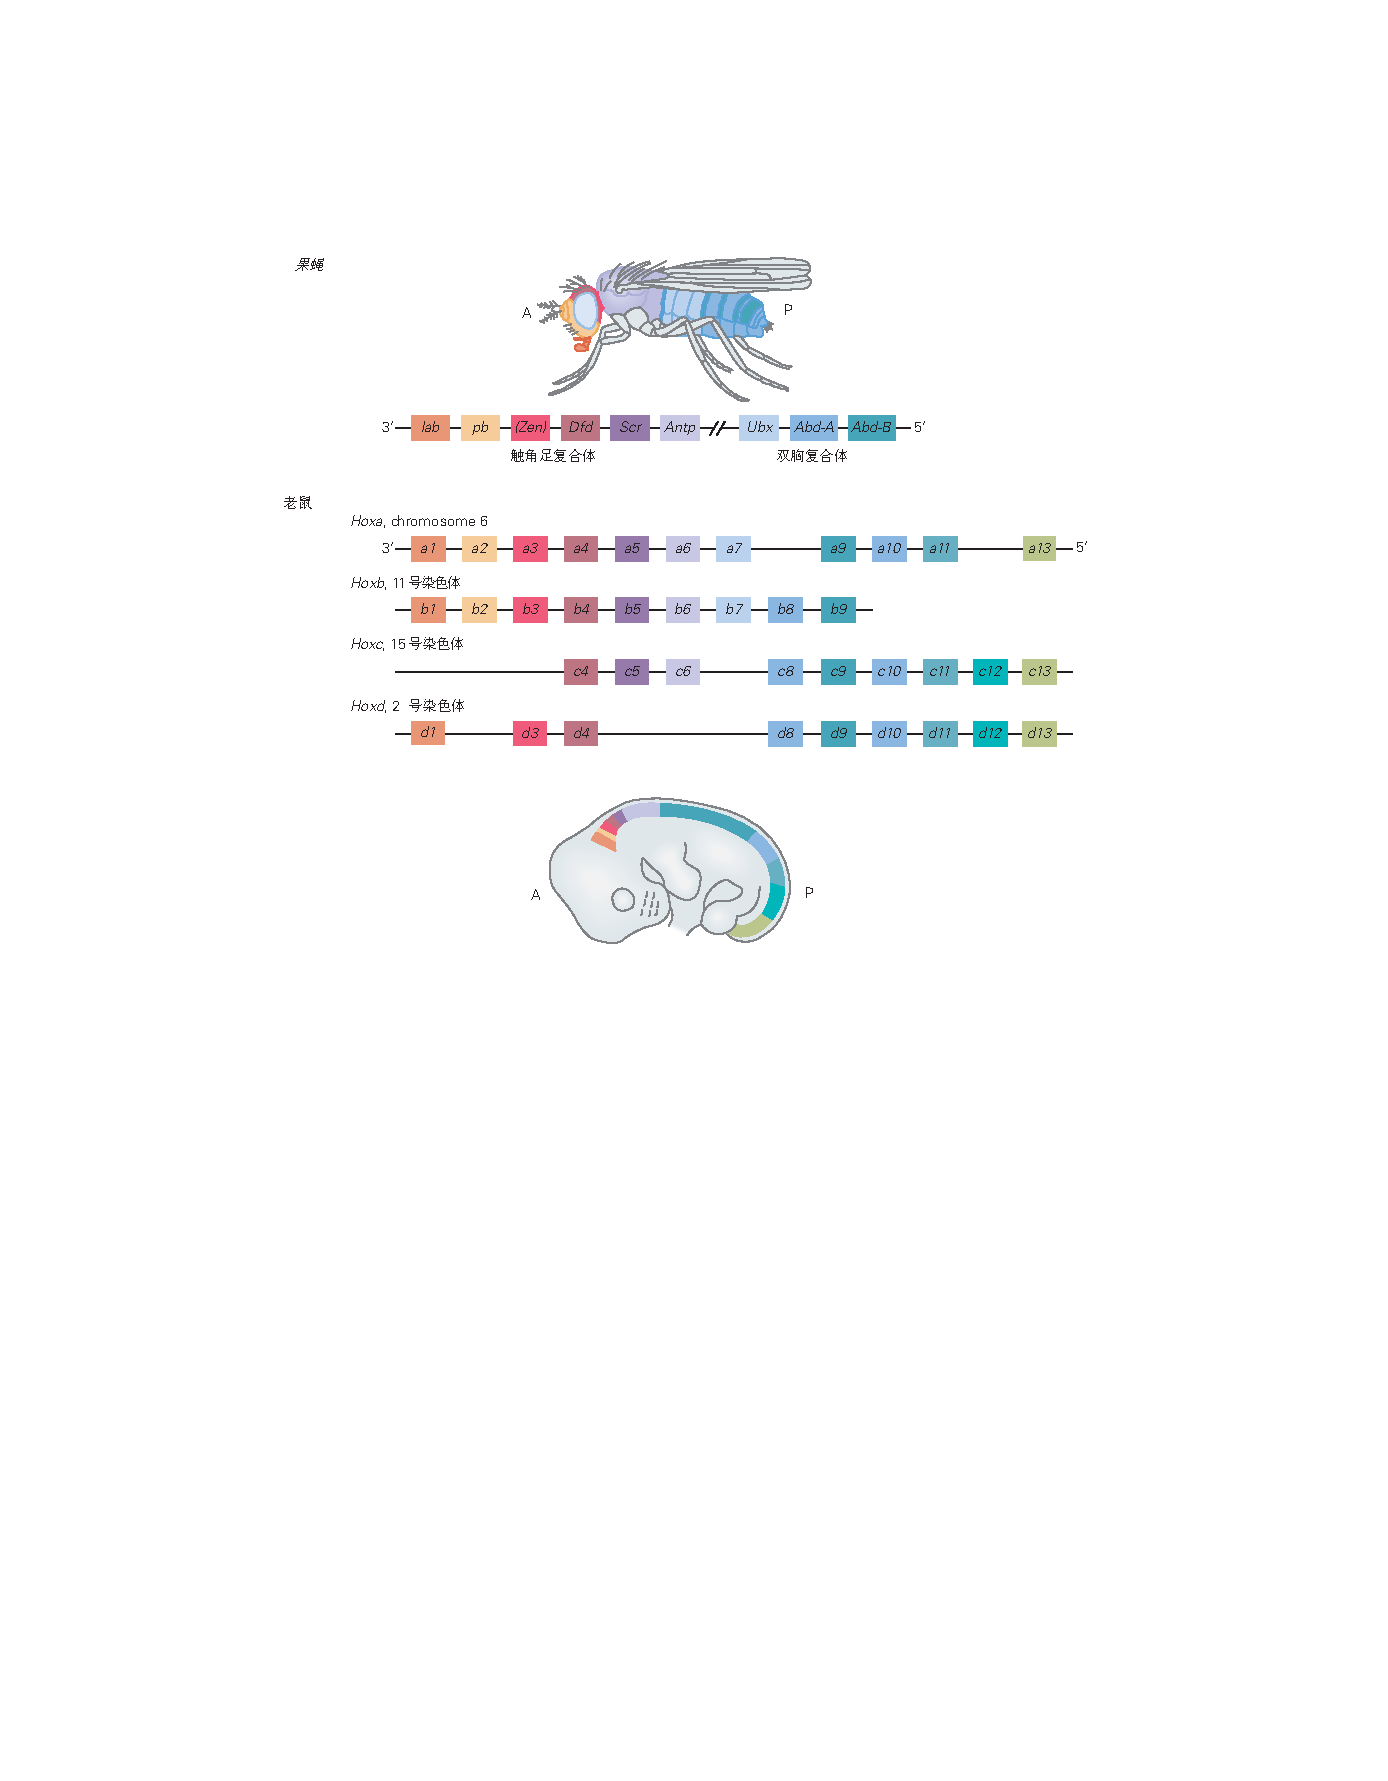
\includegraphics[width=0.7\linewidth]{chap45/fig_45_11}
	\caption{Hox 基因的簇状组织从果蝇到脊椎动物都是保守的。 该图显示了小鼠 Hox 基因和果蝇 HOM-C 基因的染色体排列。 昆虫有一个祖先的 Hox 基因簇,而鸟类和哺乳动物等高等脊椎动物有四个重复的 Hox 基因簇。 给定的 Hox 或 HOM-C 基因在染色体簇上的位置通常与该基因表达的前后体轴上的位置有关。 (经许可改编自 Wolpert 等人,1998 年。许可通过 Copyright Clearance Center, Inc. 传达。)}
	\label{fig:45_11}
\end{figure}

脊椎动物 Hox 基因家族的成员在沿发育中脑、后脑和脊髓的 rostrocaudal 轴的重叠域中表达。 与在果蝇中一样,单个 Hox 基因在其簇中的位置预测其在神经管内的表达域。 在大多数但不是所有情况下,位于染色体簇内更多 3' 位置的 Hox 基因在中脑和后脑内更多的延髓区域表达,而更多 5' 位置的基因在脊髓内逐渐更多的尾部位置表达 (图 \ref{fig:45_10} 和 \ref{fig:45_11})。 这种 Hox 基因表达的空间阵列决定了神经元多样性的许多方面。

主要在小鼠中进行的遗传研究揭示了 Hox 基因如何控制后脑和脊髓中的运动神经元特性。 我们在上面看到 Hox 基因有助于菱形节的形成,菱形节是后脑的基本细胞构建块。 后来,相同的基因有助于确定菱形节内运动神经元的身份。 例如,Hoxb1 在菱形节 4(产生面部运动神经元的结构域)中高水平表达,但在菱形节 2(产生三叉神经运动神经元的结构域)中不存在(图 \ref{fig:45_10})。

在小鼠中,消除 Hoxb1 活性的突变改变了 rhombomere 4 中细胞的命运; 从该域中出现的运动神经元的身份和连接性发生了变化。 
在没有 Hoxb1 功能的情况下,菱形节 4 中的细胞会产生支配三叉神经而不是面部目标的运动神经元,即通常在菱形节 2 中产生的运动神经元亚型(图 \ref{fig:45_12})。 
许多其他研究证实了后脑运动神经元身份受 Hox 基因表达空间分布控制的一般原则。

\begin{figure}[htbp]
	\centering
	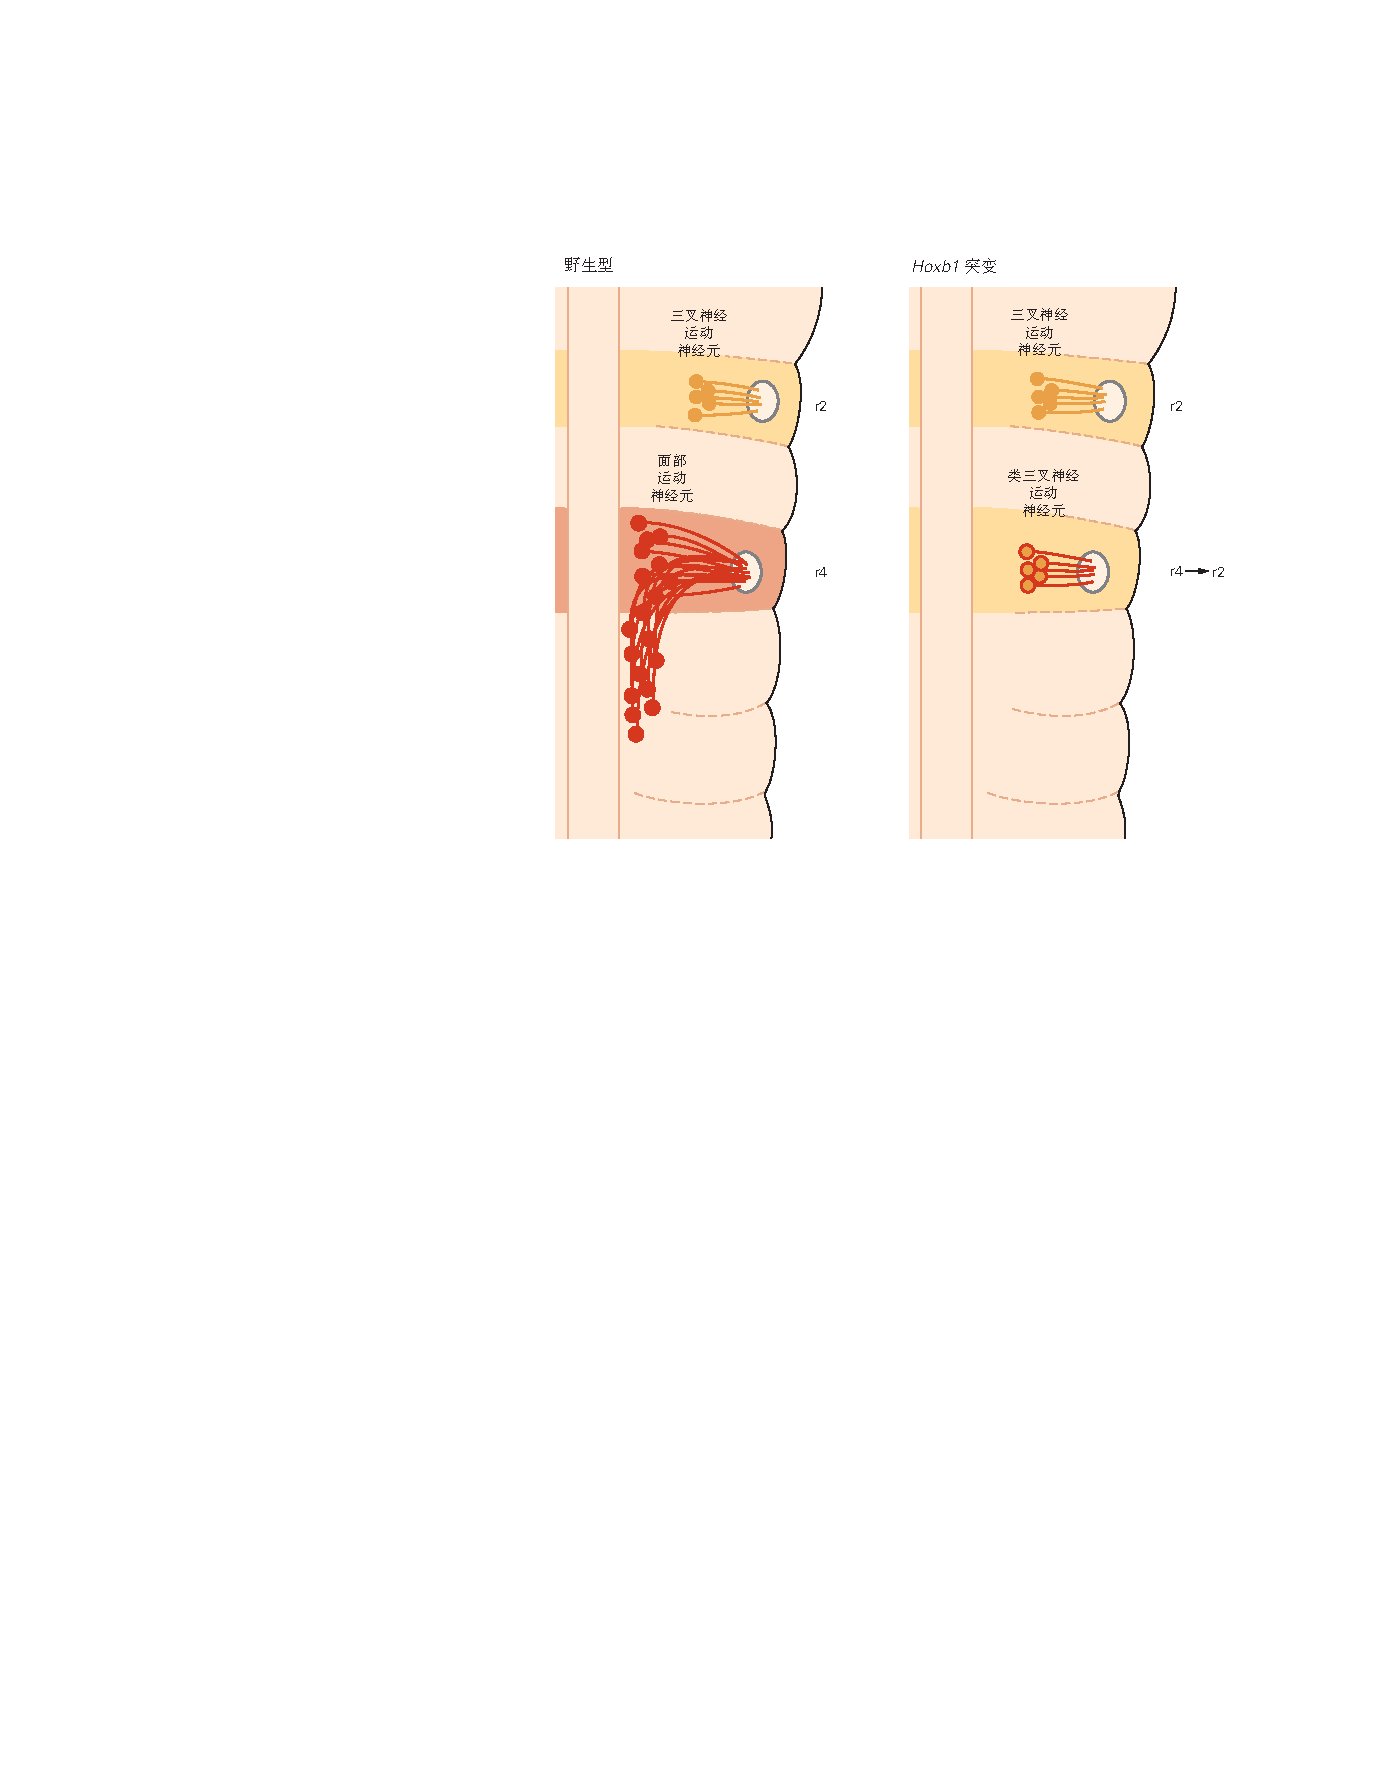
\includegraphics[width=0.75\linewidth]{chap45/fig_45_12}
	\caption{小鼠 Hoxb1 基因控制后脑运动神经元的识别和投射。 Hoxb1 通常由菱形节 r4 中的细胞以最高水平表达。 在野生型小鼠中,三叉神经运动神经元在菱形节 r2 中生成,它们的细胞体在将轴突从后脑 r2 水平伸出之前横向迁移。 相比之下,rhombomere r4 中产生的面部运动神经元的细胞体向尾部迁移,但在 r4 水平将它们的轴突投射出后脑。 在小鼠 Hoxb1 突变体中,rhombomere r4 中产生的运动神经元横向而不是尾部迁移,获得 r2 级三叉神经运动神经元的特征。 椭圆表示轴突出口点。 (经许可改编自 Struder 等人,1996 年。版权所有 © 1996 Springer Nature。)}
	\label{fig:45_12}
\end{figure}

脊髓运动神经元同一性的控制更为复杂。 脊髓运动神经元聚集在占据离散节段位置的纵向列内,与其外围目标对齐。 支配前肢和后肢肌肉的运动神经元分别存在于脊髓颈椎和腰椎水平的外侧运动柱中。 相反,支配交感神经元靶标的运动神经元位于脊髓胸段的节前运动柱内。 在外侧运动柱内,支配单个肢体肌肉的运动神经元聚集在一起形成离散的组,称为运动池。 由于高等脊椎动物的每个肢体包含 50 多个不同的肌肉群,因此需要相应数量的运动池。

脊髓中运动神经元的特性受 Hox 基因的协调活动控制,这些基因位于染色体 Hox 簇内更多的 5' 位置。 例如,Hox6 和 Hox9 蛋白的表达和活性空间域确定了臂外侧运动柱和神经节前运动柱中运动神经元的特性。 Hox6 蛋白指定臂外侧运动柱标识,而 Hox9 蛋白指定节前运动柱标识。 
前肢和胸部区域边界的运动神经元获得明确的柱状特征,因为 Hox6 和 Hox9 蛋白相互抑制(图 \ref{fig:45_13}A),类似于脊髓背腹侧模式中发生的转录交叉抑制。

\begin{figure}[htbp]
	\centering
	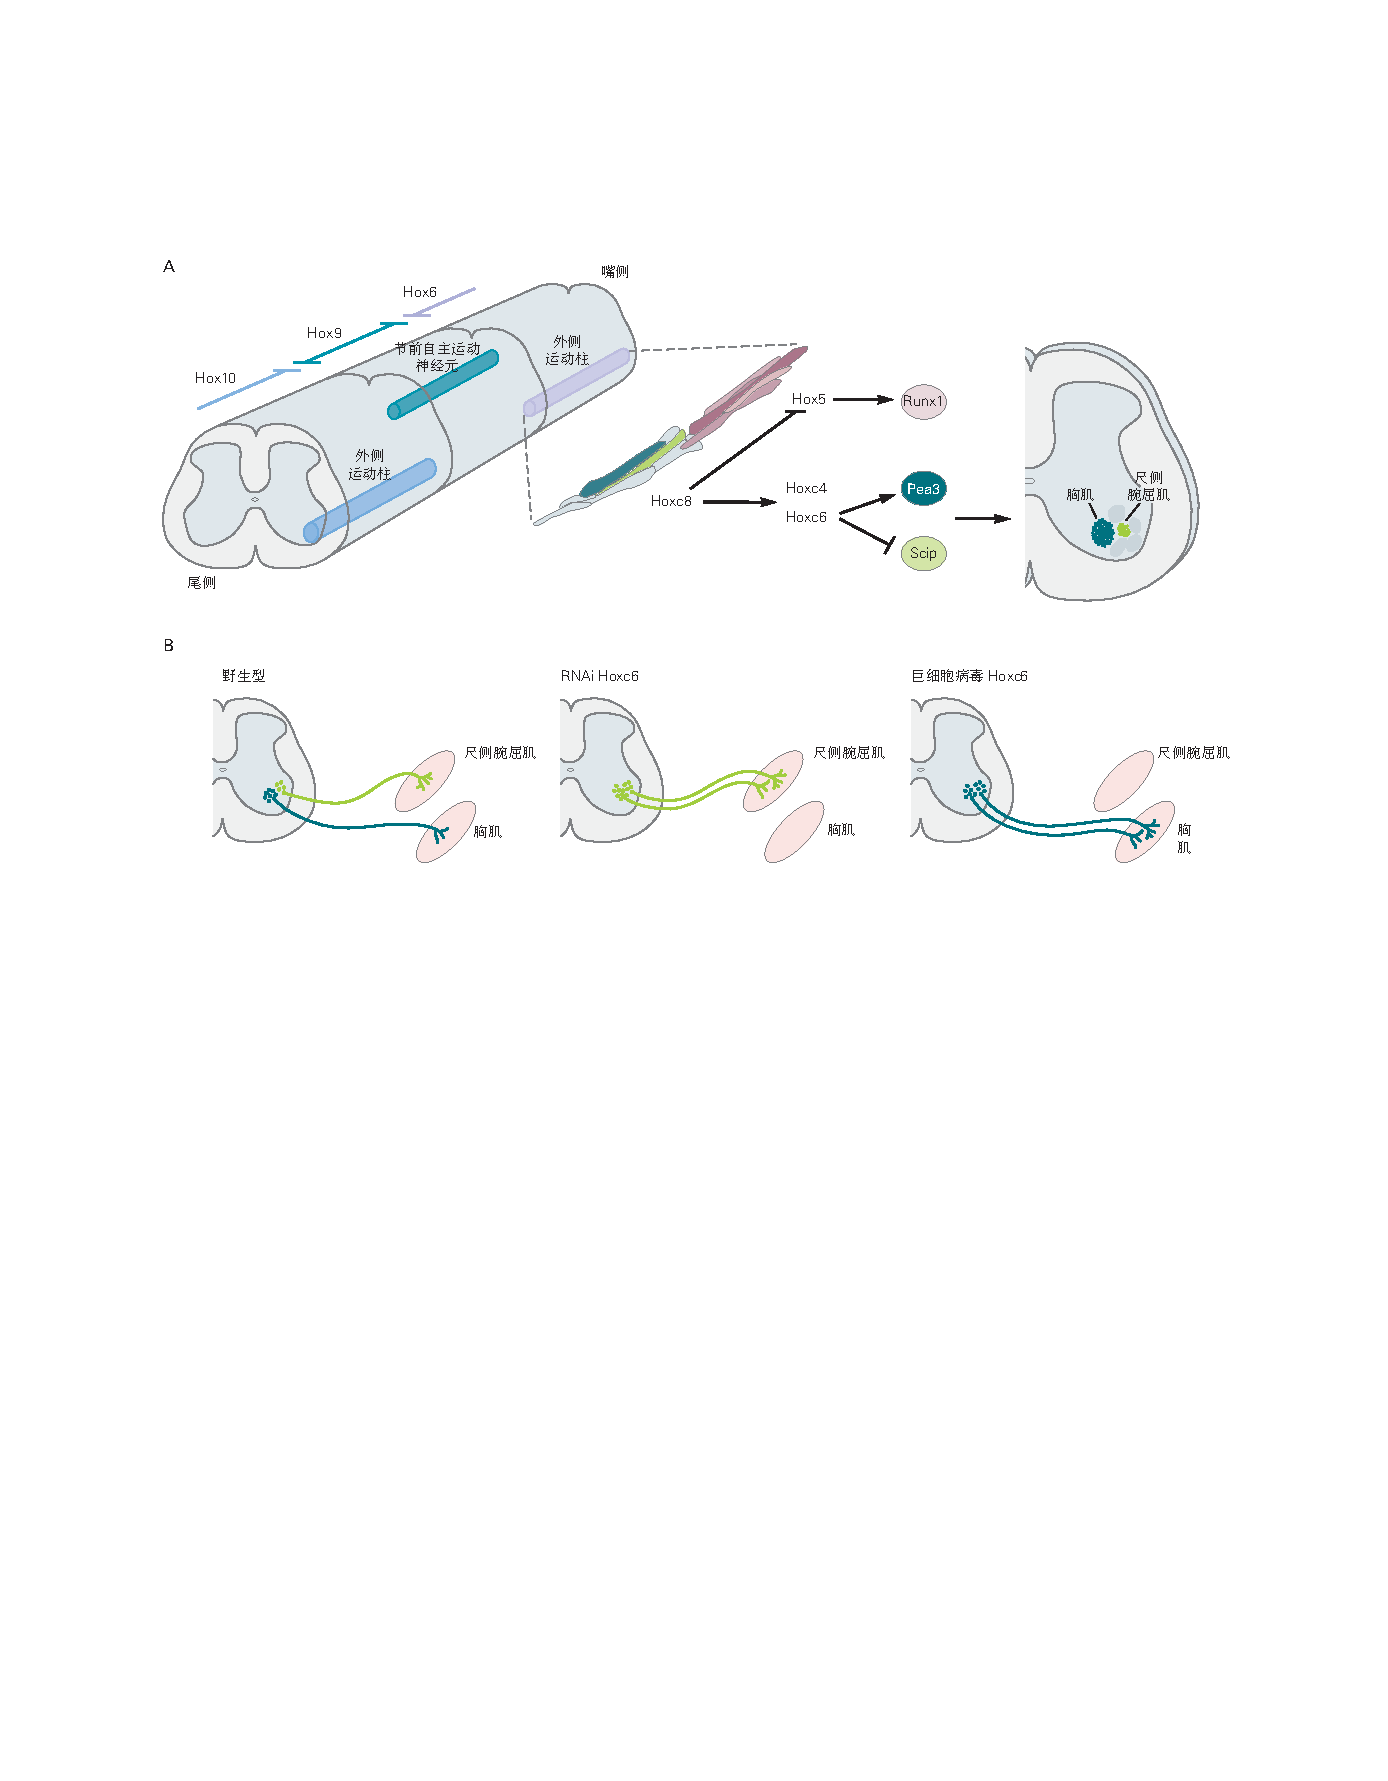
\includegraphics[width=0.95\linewidth]{chap45/fig_45_13}
	\caption{Hox 蛋白控制运动柱和池中神经元的特性。 (经许可改编自 Dasen 等人,2005 年。)A. Hox6、Hox9 和 Hox10 蛋白在脊髓不同的头尾水平的运动神经元中表达,并直接运动神经元身份和外周目标连接。 Hox6 活动控制臂外侧运动柱 (LMC) 中细胞的特性,Hox9 控制节前柱 (PGC) 中细胞的特性,而 Hox10 控制腰柱 (LMC) 中细胞的特性。 Hox6、Hox9 和 Hox10 蛋白之间的交叉抑制相互作用完善了 Hox 谱,Hox 激活剂功能定义了 LMC 和 PGC 身份。 一个更复杂的 Hox 转录网络控制着运动池的身份和连接。 Hox 基因决定了 LMC 内运动池的 rostrocaudal 位置。 尾部 LMC 神经元需要 Hoxc8 来产生胸大肌 (Pec) 和尺侧腕屈肌 (FCU) 肌肉的运动池; 这些神经元分别表达转录因子 Pea3 和 Scip。 Pec 和 FCU 池中 Hox 表达的模式是通过转录网络建立的,该网络似乎主要由 Hox 交叉抑制相互作用驱动。 B. 改变运动池内的 Hox 代码会改变肌肉连接的模式。 Hox6 表达谱的改变决定了 Pea3 和 Scip 的表达,并控制运动轴突投射到 Pec 或 FCU 肌肉。 Hox6 的 RNA 干扰 (RNAi) 敲低抑制了 Pec 肌肉的神经支配,因此运动轴突仅支配 FCU 肌肉。 由巨细胞病毒 (CMV) 启动子驱动的 Hoxc6 的异位表达抑制与 FCU 的连接,因此运动轴突仅支配 Pec 肌肉。}
	\label{fig:45_13}
\end{figure}


\subsection{局部信号和转录回路进一步使运动神经元亚型多样化}
外侧运动柱内的运动神经元如何发展出更精细的特征,将它们的轴突引导到特定的肢体肌肉? 再次,Hox 基因控制运动神经元多样化的这个阶段。 我们通过考虑在支配前肢肌肉的臂外侧运动柱内产生神经元的不同分裂和集合特性的途径来说明 Hox 蛋白的这种功能(图 \ref{fig:45_13}A)。

由不同横向运动柱中的神经元表达的 Hox 蛋白之间的抑制相互作用确保填充不同运动池的神经元表达不同的 Hox 蛋白表达谱。 这些 Hox 配置文件指导下游转录因子以及轴突表面受体的表达,使运动轴突能够响应肢体内的局部线索,引导它们到达特定的肌肉目标。 例如,Hox6 蛋白的表达激活视黄酸信号通路,该通路指导两个同源域转录因子 Is11 和 Lhx1 的表达。 这些因素反过来将运动神经元分配到两个分区类别,并确定引导肢体运动轴突的肝配蛋白受体的表达模式。 
在肝配蛋白信号的控制下,这两个部分的运动神经元轴突投射到肢体间充质的腹侧和背侧(图 \ref{fig:45_14})。

\begin{figure}[htbp]
	\centering
	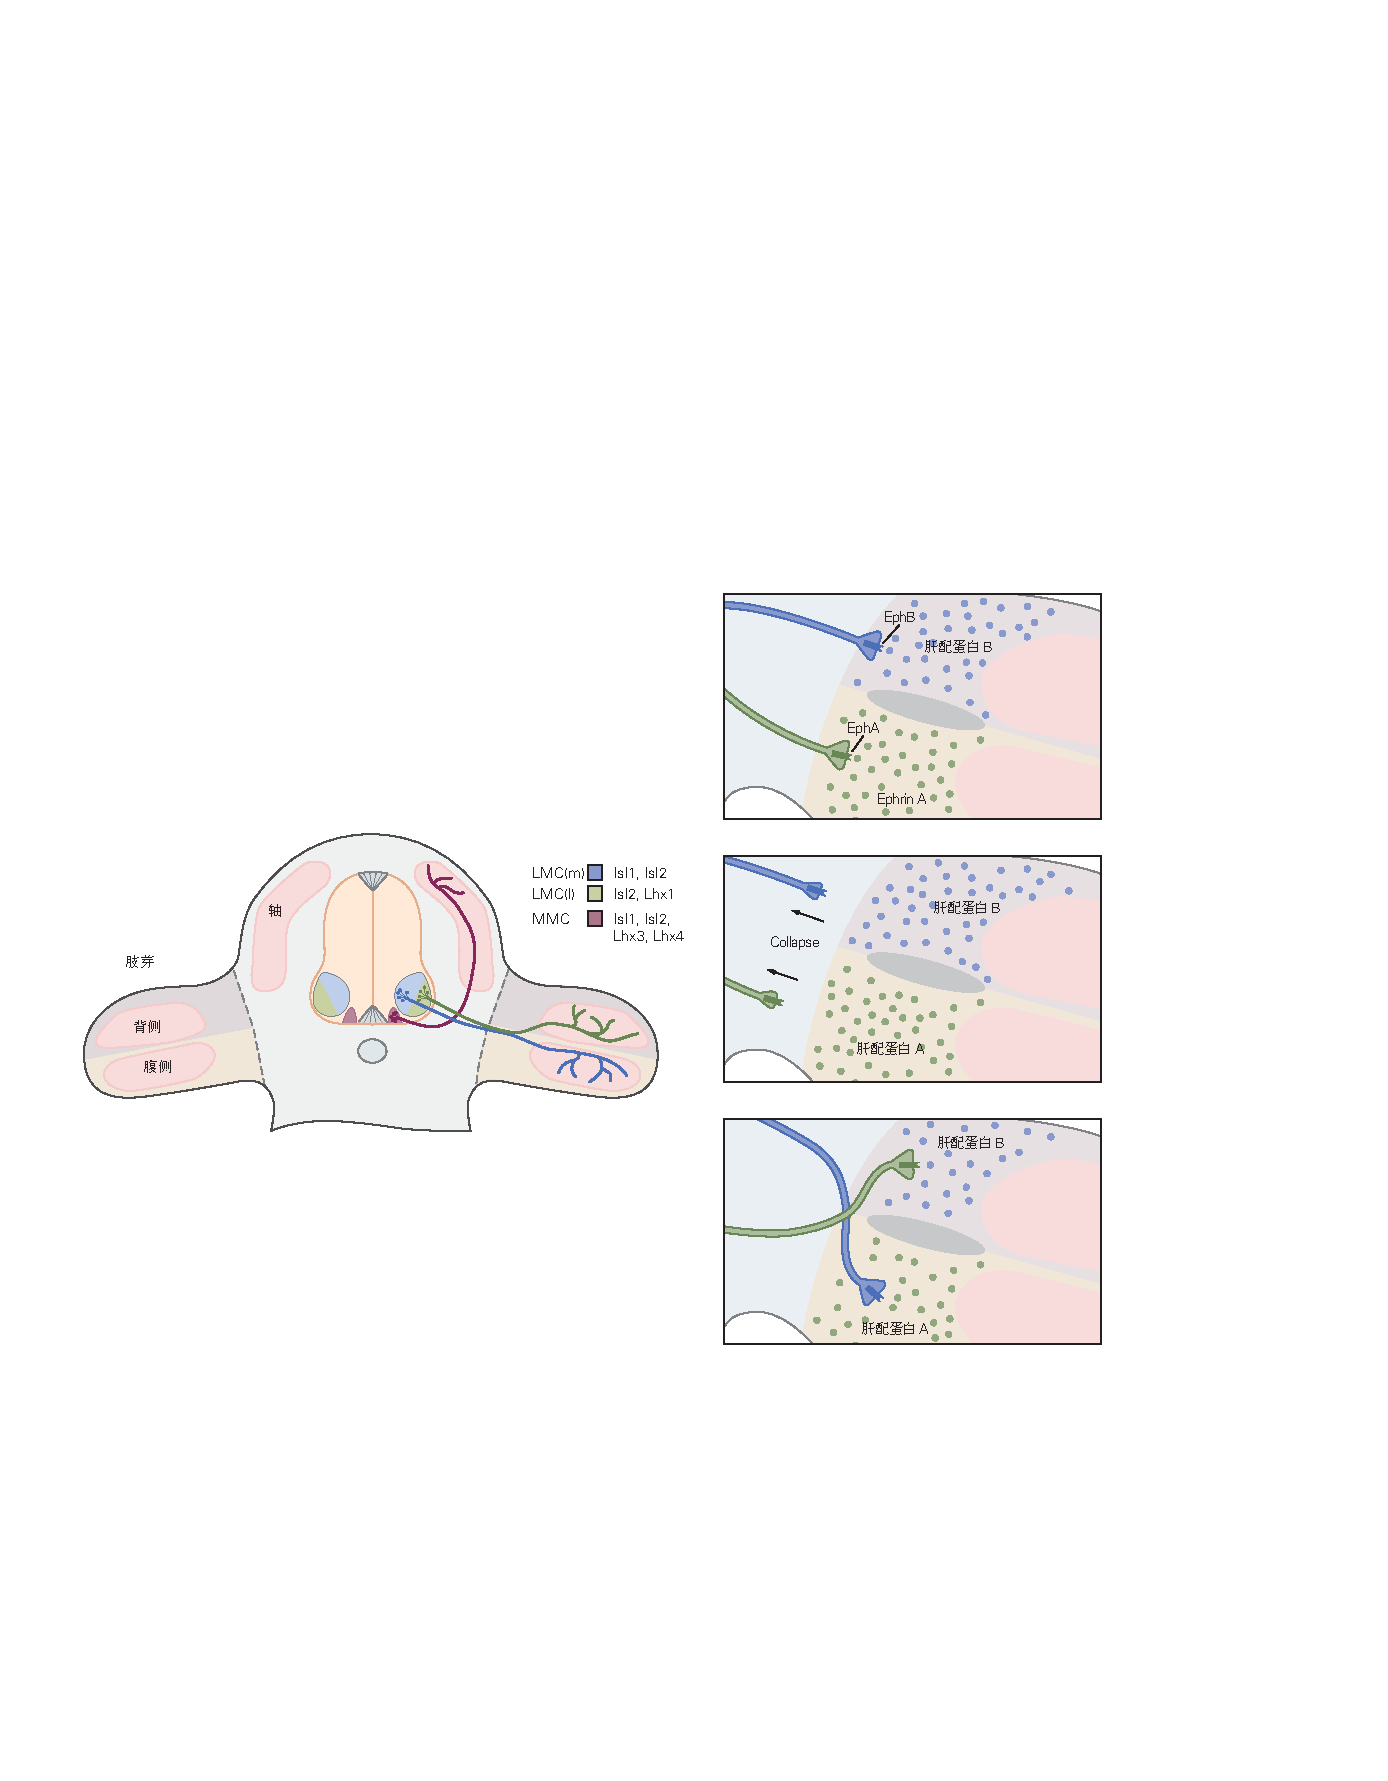
\includegraphics[width=0.65\linewidth]{chap45/fig_45_14}
	\caption{肝配蛋白类酪氨酸激酶受体引导外侧运动柱神经元的轴突进入肢体。 外侧运动柱 (LMC) 的内侧和外侧分裂中的运动神经元分别将轴突投射到肢体间充质的腹侧和背侧。 LIM 类同源结构域蛋白的表达谱调节这种背腹投射。 由内侧 LMC 神经元表达的 LIM 同源域蛋白 Isl1 指导 EphB 受体的高水平表达,因此当这些细胞的轴突进入肢体时,它们被细胞表达的高水平排斥肝配蛋白 B 配体阻止向背投射 背肢间充质。 因此,这些轴突投射到腹侧肢体间充质中。 相反,由外侧 LMC 神经元表达的 LIM 同源域蛋白 Lhx1 指导 EphA 受体的高水平表达,因此当这些细胞的轴突进入肢体时,它们被高水平表达的排斥肝配蛋白 A 配体阻止向腹侧投射 由腹侧肢体间质细胞产生。 因此,这些轴突投射到背肢间充质中。 Eph 和 ephrin 信号在第 \ref{chap:chap47} 章中有更详细的讨论。(缩写:MMC,内侧运动柱。)}
	\label{fig:45_14}
\end{figure}

然而,并非所有运动神经元列都由 Hox 蛋白活性决定。 中位运动柱在脊髓的所有节段水平产生,与轴向肌肉对齐。 中位运动柱细胞的发育受脊髓腹侧中线分泌的 Wnt4/5 信号和同源域蛋白 Lhx3 和 Lhx4 的表达控制,这使得该柱中的神经元对 Hox 蛋白的节段性模式作用免疫。

因此,在后脑和脊髓中,运动神经元与特定肌肉的点对点连接是通过同源域蛋白表达和活动的紧密协调程序出现的。 在脊椎动物中,这些基因已经进化为指导神经元亚型和连通性以及基本的身体计划。


\section{发育中的前脑受内在和外在影响的影响}
哺乳动物前脑中的神经元形成调节情绪行为、感知和认知的回路,并参与记忆的存储和检索。 与后脑非常相似,胚胎前脑最初沿其 rostrocaudal 轴分为称为前体的横向组织区域。 前粒 1 至 3 发育成间脑的尾部,丘脑从中出现。 前粒 4 至 6 产生头端间脑和端脑。 头侧间脑的腹侧区域产生下丘脑和基底神经节,而端脑产生新皮质和海马体。

\subsection{感应信号和转录因子梯度建立区域分化}
最后,我们转向新皮层本身的模式,询问支配中枢神经系统其他区域发育的发育机制和原则是否也控制专门负责特定感觉、运动和认知功能的皮层区域的出现。

从20世纪初布罗德曼的经典解剖学描述开始,我们就知道大脑皮层被细分为许多不同的区域。 最近对皮层发育的研究已经开始深入了解建立体感、听觉和视觉区域的信号机制。

现在有证据表明存在皮质“原型图”,这是一种基本计划,其中在其他大脑区域的输入影响发育之前,在发育早期建立不同的皮质区域。 对发育中的新皮层中转录因子表达的研究支持了这一观点。 两个同源域转录因子 Pax6 和 Emx2 在发育中的新皮层的心室区以互补的前后梯度表达——前部水平高水平的 Pax6 和后部水平高水平的 Emx2。 
这些早期模式部分是由 FGF 信号的局部延髓源建立的,它促进 Pax6 并抑制 Emx2 表达(图 \ref{fig:45_15}A)。 
与后脑的情况一样,Pax6 和 Emx2 表达的不同空间域因两种转录因子之间的交叉抑制相互作用而变得尖锐。

\begin{figure}[htbp]
	\centering
	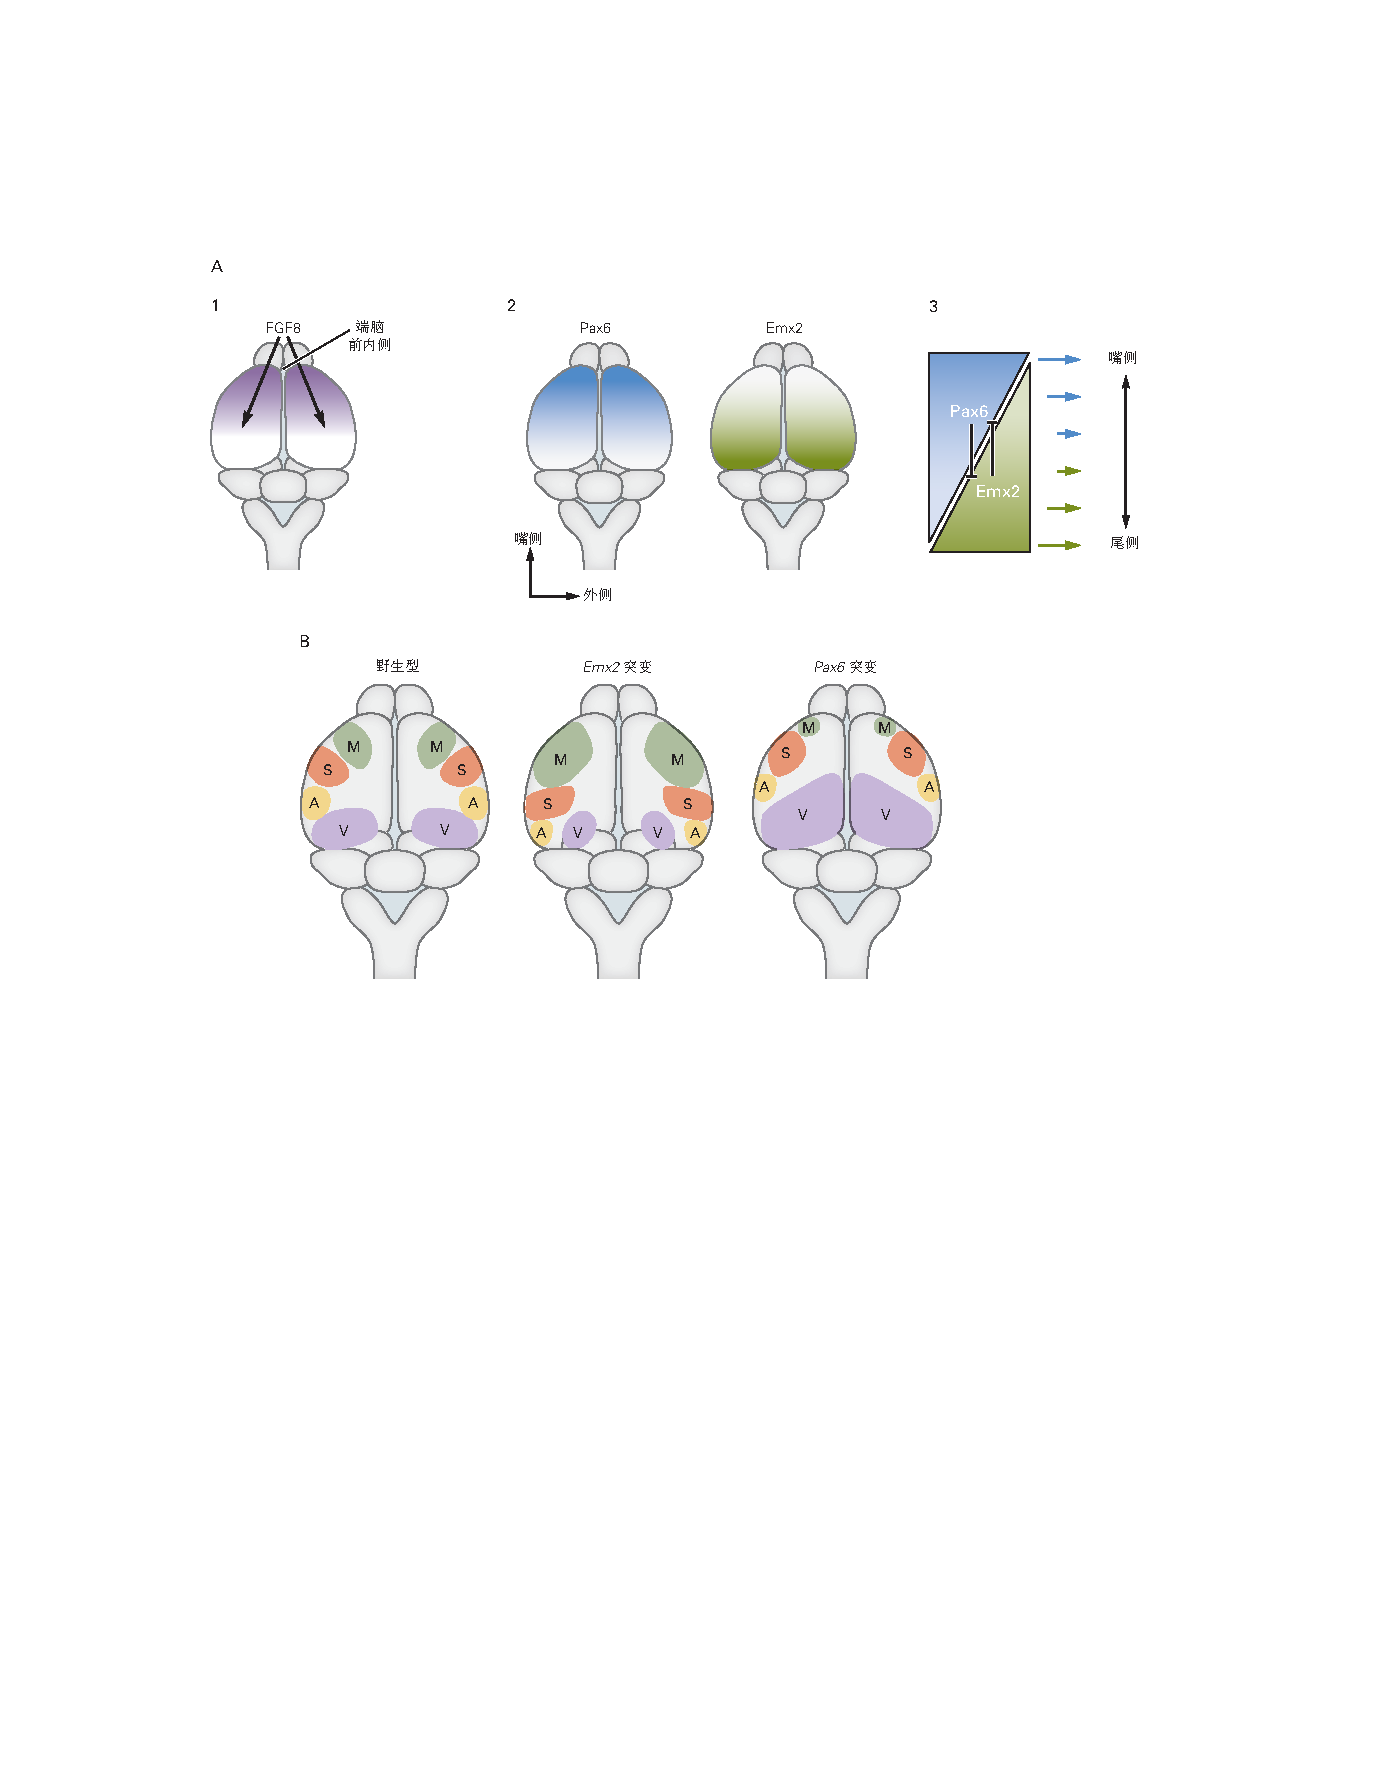
\includegraphics[width=0.9\linewidth]{chap45/fig_45_15}
	\caption{转录因子表达的前后梯度沿发育前脑的前后轴建立离散的功能区。 (改编自 Hamasaki 等人,2004 年。) A. (1) 来自前内侧端脑的 FGF8 信号建立了大脑皮层的头尾模式。 (2) 小鼠大脑皮层发育的自上而下视图显示了转录因子 Pax6 和 Emx2 的反向 rostrocaudal 梯度。 (3) 这两个转录因子相互抑制对方的表达。 B. 不同的功能区在不同的 rostrocaudal 位置发展。 运动区在前部区域 (M) 发育,视觉区在更多的后部区域 (V) 发育。 Emx2 功能的遗传消除导致运动区域的扩展和听觉 (A) 和视觉区域的收缩。 相反,消除 Pax6 功能会导致视觉区域扩大以及运动和听觉区域收缩。 (缩写:S,体感区。)}
	\label{fig:45_15}
\end{figure}

Pax6 和 Emx2 的空间分布有助于建立新皮质的初始区域模式。 在缺乏 Emx2 活性的小鼠中,头侧新皮层(运动和体感区域)以更多的尾部听觉和视觉区域为代价扩大。 相反,在缺乏 Pax6 活性的小鼠中,视觉和听觉区域以运动和体感区域为代价扩大(图 \ref{fig:45_15}B)。

因此,与脊髓、后脑和中脑一样,早期新皮质模式是通过局部感应信号和转录因子表达梯度之间的相互作用建立的。 这些梯度如何指定新皮质中的离散功能区域仍不清楚。 与后脑中的分割不同,其中转录因子精确指定菱形节,单个新皮层区域的转录标记尚未确定。

\subsection{传入输入也有助于区域化}
在成人新皮质中,不同的功能区域可以通过神经元分层模式(区域的细胞结构)及其神经元连接的差异来区分。 细胞模式区域差异性的一个显着实例是啮齿动物初级体感皮层中的神经元和神经胶质细胞的网格状阵列,称为“桶”。 
每个皮质桶从鼻子上的单个胡须接收体感信息,皮质桶的规则排列反映了来自体表的传入信息的躯体组织,最终将丘脑传出神经投射到特定的皮质桶(图 \ref{fig:45_16}A) 。

\begin{figure}[htbp]
	\centering
	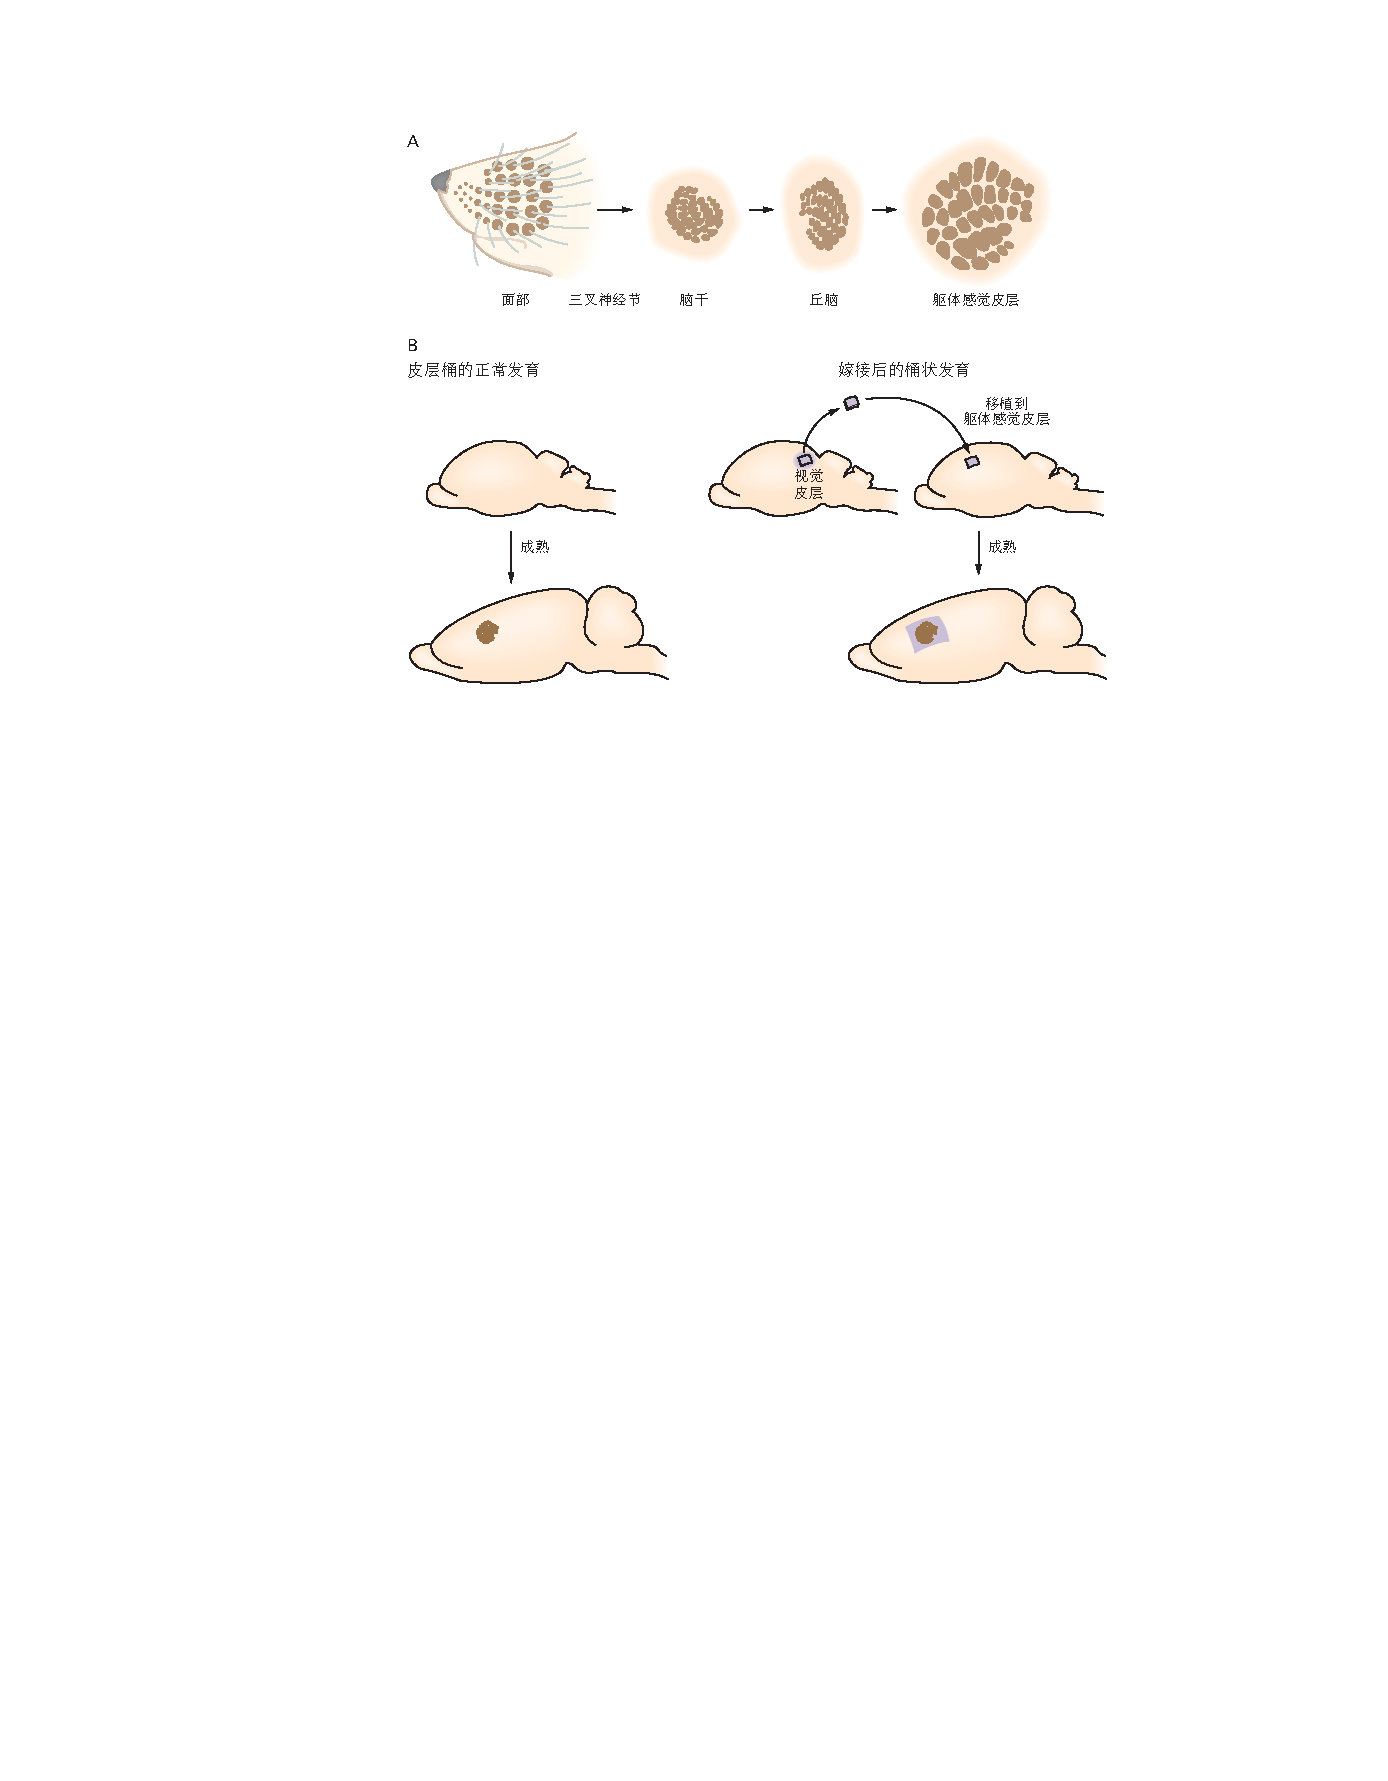
\includegraphics[width=0.7\linewidth]{chap45/fig_45_16}
	\caption{感觉输入调节啮齿动物发育中的体感皮层中“桶”的组织。 (改编自 Schlaggar 和 O’Leary 1991。) A. 啮齿动物体感皮层的桶状区域形成动物鼻子上成排胡须的躯体表征。 胡须场的类似表现存在于上游——在脑干和丘脑核中,它们将体感输入从面部传递到皮层。 B. 桶状细胞组织在视觉皮层组织的发育过程中被诱导,该组织在出生后早期被移植到体感皮层中。}
	\label{fig:45_16}
\end{figure}

皮质桶在出生后不久就很明显,它们的发育取决于外围传入输入的关键时期; 如果在这个关键时期消除了皮肤中的晶须场,它们的形成就会中断。 引人注目的是,如果预期的视觉皮层组织在出生前后被移植到体感皮层中,则在移植组织中会形成桶状结构,其图案与正常体感桶状区域非常相似(图 \ref{fig:45_16}B)。 总之,这些发现表明传入输入将新皮质模式的各个方面叠加在原型图的基本特征上。

输入到不同皮层区域的性质会影响神经功能和细胞结构。 这可以通过在将一种感觉方式的传入通路重新路由到通常处理不同方式的新皮质区域后监测生理和行为反应来证明。 
在视网膜输入被重新路由到听觉通路的动物中,初级听觉皮层包含视觉空间而不是声音频率的系统表征(图 \ref{fig:45_17})。 
当这些动物被训练来区分视觉和听觉提示时,当重新连接的听觉皮层被视觉激活时,它们会将提示视为视觉提示。

\begin{figure}[htbp]
	\centering
	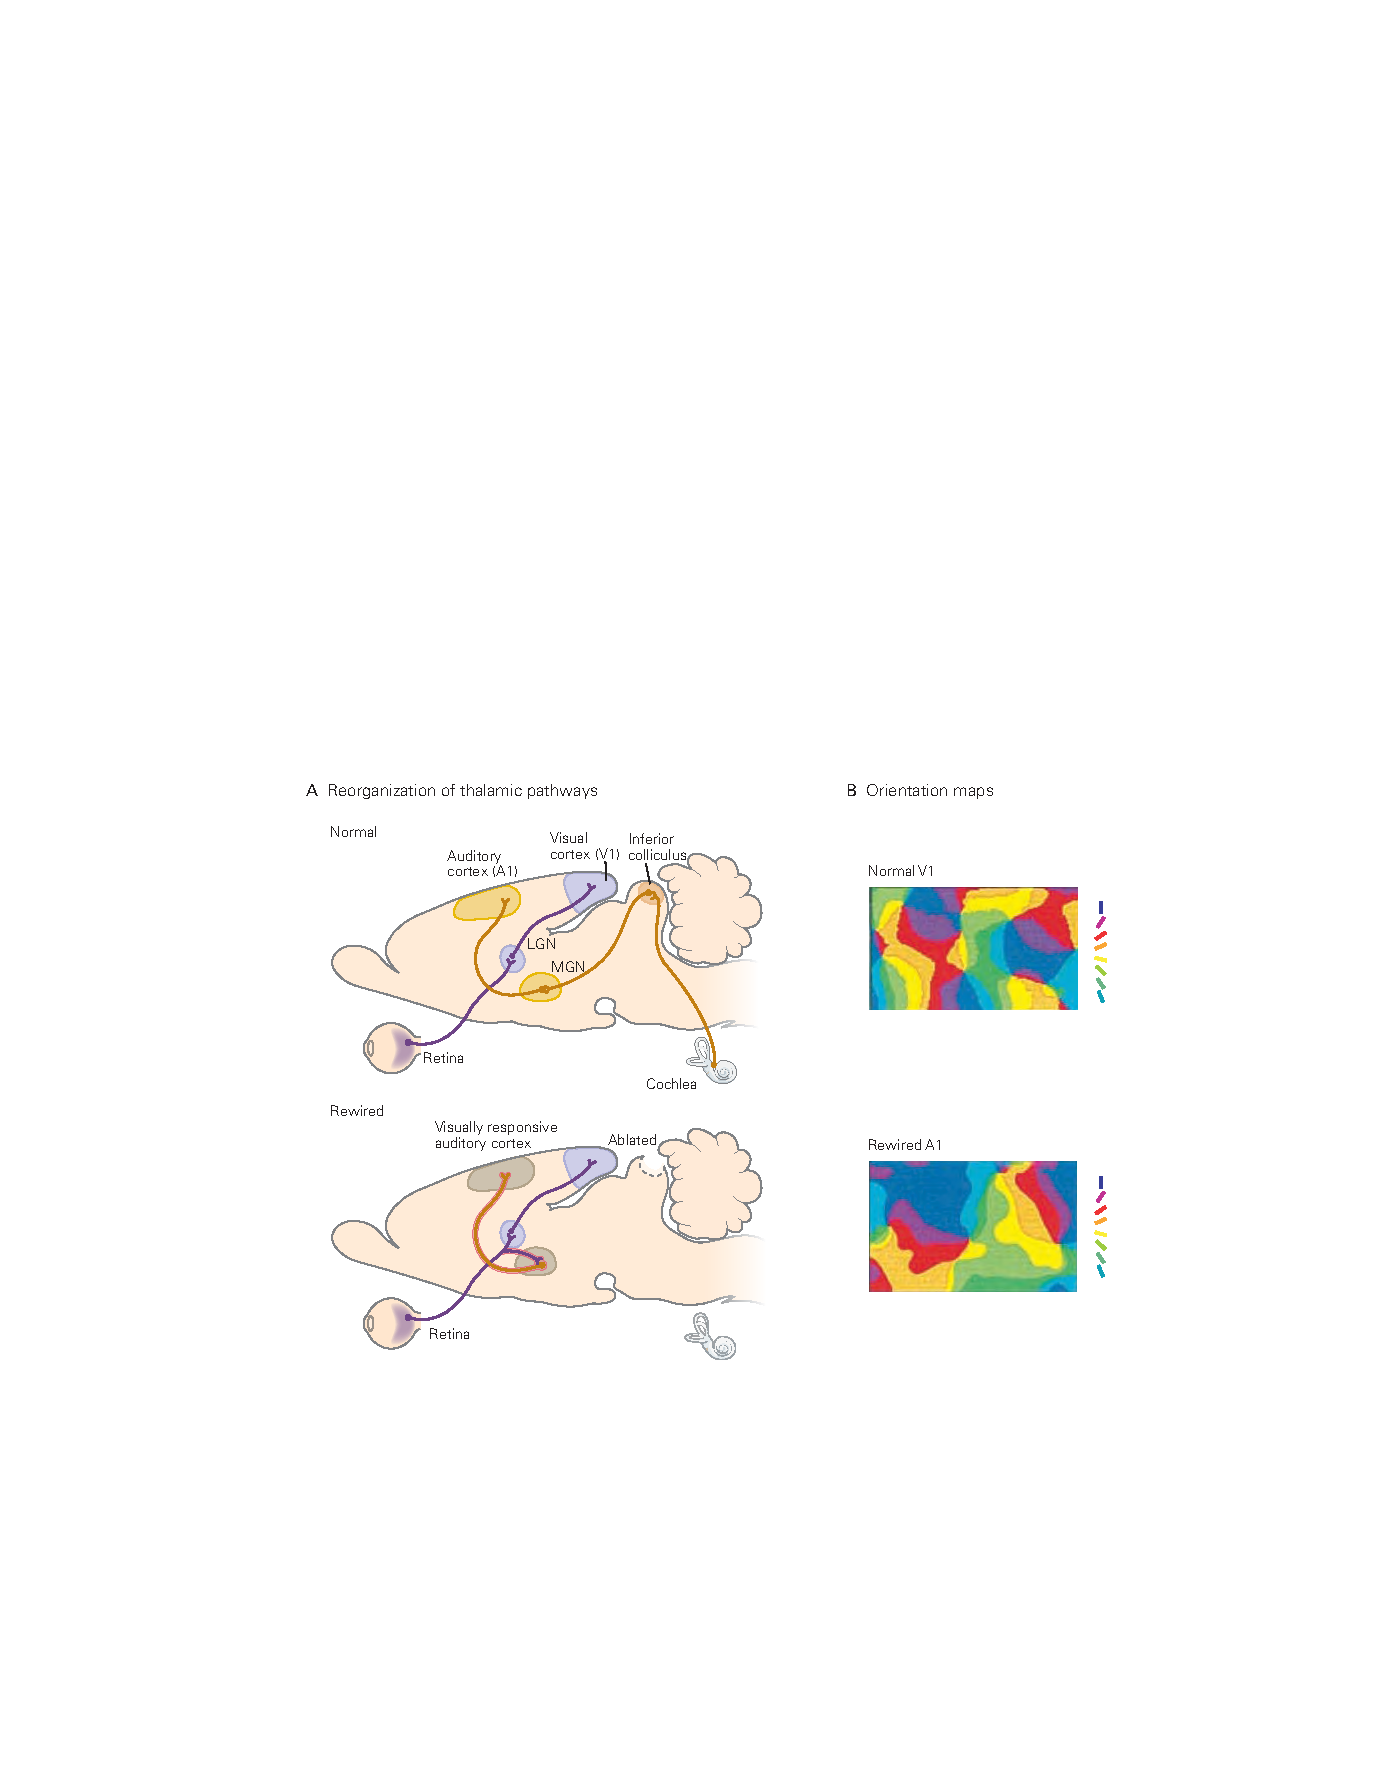
\includegraphics[width=0.8\linewidth]{chap45/fig_45_17}
	\caption{重新路由丘脑皮层输入可以为新的感觉功能募集皮层区域。 (经许可改编自 Sharma、Angelucci 和 Sur 2000。版权所有 © 2000 Springer Nature。) A. 视觉通路由来自视网膜的传入纤维组成,这些纤维支配外侧膝状体核 (LGN) 和上丘。 从 LGN 项目到初级视觉皮层 (V1) 的轴突。 听觉通路从耳蜗核(未显示)投射到下丘,然后投射到内侧膝状体核 (MGN) 和初级听觉皮层 (A1)。 消融新生雪貂的下丘会导致视网膜传入神经支配 MGN。 因此,听觉皮层被重新编程以处理视觉信息。 B. 使用固有信号的光学成像,在雪貂的重新布线的 A1 听觉皮层中观察到与正常 V1 皮层中看到的相似的视觉方向图。 不同的颜色代表不同的受体场方向(见条形图}
	\label{fig:45_17}
\end{figure}

因此,大脑通路和新皮层区域是在早期发育过程中通过遗传程序建立的,但后来它们的特殊解剖学、生理学和行为功能取决于传入输入。


\section{要点}
1. 早期脊椎动物胚胎由三层细胞组成——外胚层、中胚层和内胚层。 整个神经系统起源于外胚层,更具体地说,起源于称为神经板的外胚层中央条带。 

2. 外胚层内神经板的形成通过称为诱导的过程发生,其中底层的中胚层细胞分泌可溶性因子,诱导邻近外胚层细胞中基因表达的神经程序。 诱导涉及一种“去抑制”机制,其中中胚层衍生的可溶性因子阻止外胚层衍生的骨形态发生蛋白(BMP;转化生长因子 β 家族的成员)抑制神经命运。 

3. 诱导后,神经板从外胚层内陷形成神经管。 管产生中枢神经系统,而神经管和外胚层之间边界处的细胞形成神经嵴,神经嵴通过胚胎迁移形成周围神经系统的感觉和自主神经节。 

4. 神经管一形成,就开始区域化。 沿前后轴的区域化导致一系列细分。 前区成为大脑,后区成为脊髓。 预期大脑的分裂产生前脑、中脑和后脑。 前脑进一步分裂形成端脑,皮质、海马体和基底神经节由此产生; 和间脑,产生丘脑、下丘脑和视网膜。 后脑在前方分裂形成脑桥和小脑,在后方形成延髓。 

5. 前后模式由 Wnt 信号的梯度建立,其产生于后部 Wnt 的选择性产生和前部 Wnt 抑制剂的选择性产生。 

6. 沿前后轴的细分由位于神经管内指定位置的称为组织中心的细胞群建立。 组织中心分泌的因子会影响神经管的邻近区域,并指定其中的神经元类型。 例如,后脑和中脑边界处的峡部组织者分泌 Wnt 和成纤维细胞生长因子 (FGF)。 它们在前部和后部区域的作用不同,因为早期的模式化事件导致这些区域的细胞表达不同的转录因子。

7. 再后来,进一步细分形成前脑中的前体节和后脑中的菱形节,转录因子的差异表达导致每个神经元产生不同的类型。 

8. 在后脑和脊髓中,运动神经元根据其前后位置获得不同的特性,分化为支配不同肌肉的组。 称为 Hox 蛋白的转录因子的差异表达在运动神经元的多样化中尤为重要。 它们与其他转录因子和可溶性因子一起作用,将运动神经元分成柱状和池状,每个池都注定要支配特定的肌肉。 

9. 神经管也沿着背腹轴排列。 与前后区域化类似,图案化是由形态发生素的梯度引起的。 最重要的是形成腹侧高-背侧低梯度的声波刺猬 (Shh) 和形成背侧高-腹侧低梯度的 BMP。 不同水平的 Shh 和 BMPs 诱导不同的转录因子,这反过来导致不同细胞类型的产生。 

10. 将大脑皮层区域化为运动区、感觉区和关联区也始于诱导转录因子差异表达的形态发生素梯度,从而建立区域身份的“原型图”。 区域之间的相互作用以及来自皮层下区域的输入完善了原型图以形成明确的皮层区域。 

11. 几个一般原则解释了早期神经发育的许多方面: (a) 归纳相互作用导致一组统一的细胞细分为离散区域。 (b) 一小组可溶性因子,如 FGF、BMP 和 Wnt,在多个阶段多次使用以对神经系统进行区域化。 (c) 这些因子的不同水平导致不同转录因子的表达,进而产生不同的神经细胞类型。 (d) 表达不同转录因子的细胞之间的抑制相互作用使前后轴和背腹轴的边界变尖锐。 

12. 直到最近,对神经发育早期阶段的研究仅限于实验动物。 现在的最新进展使神经科学家能够使用培养的人类细胞来概括其中的一些过程。 因此,很快就有可能了解人类与其他物种之间是否存在导致人类大脑复杂性和人类大脑疾病的关键早期差异。

%\subsection{选读}
%\subsection{参考文献}
